%%% File encoding: UTF-8
%% äöüÄÖÜß  <-- no German Umlauts here? Use an UTF-8 compatible editor!

%%% Magic comments for setting the correct parameters in compatible IDEs
% !TeX encoding = utf8
% !TeX program = pdflatex
% !TeX spellcheck = en
% !BIB program = biber


\documentclass[master,english,smartquotes]{hgbthesis}
% Permissible options in [..]:
%   Type of work: diploma, master (default), bachelor, internship
%   Main language: german, english (default)
%		smartquotes: for simplified insertion of quotes (only "...")
%%%----------------------------------------------------------

\RequirePackage[utf8]{inputenc}		% Remove when using lualatex or xelatex entfernen!
\RequirePackage[T1]{fontenc}
\RequirePackage[version=4]{mhchem}
\RequirePackage{mol2chemfig}
\RequirePackage{chemfig}
\RequirePackage{multirow}
\RequirePackage{nicefrac}

% Beautify xml files
\RequirePackage{color}
\RequirePackage[usenames,dvipsnames,svgnames,table]{xcolor}
\RequirePackage{listings}
\makeatletter
\def\lst@DelimPrint#1#2{%
      #1%
      \begingroup
        \lst@mode\lst@nomode \lst@modetrue
        #2\delimstyle\lst@XPrintToken%
      \endgroup
      \lst@ResetToken
    \fi}
\makeatother
\newcommand\delimstyle{}

\lstdefinelanguage{XMLnew}{
  tag=**[s][\color{blue}\renewcommand\delimstyle{\color{black}}]<>,
  commentstyle=\color{gray},
  breaklines=true,
  morestring=[b]",
  morecomment=[s]{<!--}{-->},
  keywordstyle=\color{orange},
  stringstyle=\color{black},
}[keywords,comments,strings,html]%

%Make ((sub)sub)sections include their graphics without floating into next ((sub)sub)section.
\usepackage{placeins}
\let\Oldsection\section
\renewcommand{\section}{\FloatBarrier\Oldsection}
\let\Oldsubsection\subsection
\renewcommand{\subsection}{\FloatBarrier\Oldsubsection}
\let\Oldsubsubsection\subsubsection
\renewcommand{\subsubsection}{\FloatBarrier\Oldsubsubsection}

\graphicspath{{images/}}    % location of images and graphics
\logofile{logo.eps}	% logo file = images/logo.eps (use \logofile{} for no logo)
\bibliography{references}  	% name of bibliography file (references.bib)

%%%----------------------------------------------------------
% Title page entries
%%%----------------------------------------------------------

%%% Entries for ALL types of work: --------------------------
\title{Bistability and state switching in computational dynamic histone modification models}
\author{Michel Krecké}

%\programtype{Fachhochschul-Bachelorstudiengang}		% select/edit
\programtype{Institut für Informatik}

\programname{Professur für Bioinformatik}
\placeofstudy{Leipzig}
\dateofsubmission{2021}{07}{04}	% {YYYY}{MM}{DD}

\advisor{Prof. Dr. Sonja Prohaska}

\hyphenation{nuc-leo-some}
\hyphenation{nuc-leo-somes}
\hyphenation{pre-dom-in-ant}


%\strictlicense		%%% restrictive license instead of Creative Commons (discouraged!)

%%%----------------------------------------------------------
\begin{document}
%%%----------------------------------------------------------

%%%----------------------------------------------------------
\frontmatter							% title part (roman page numbers)
%%%----------------------------------------------------------

\maketitle
\tableofcontents

% \chapter{Preface}




 	% preface is optional
% \chapter{Abstract}
Main question: How to establish bistability with EpiDynast?
	next neighbour not enough (how to prove?)
	how to find all the possibilities to establish bistability?
		(Mathematical) basis for bistability\\

This should be a 1-page (maximum) summary of your work in English.


% \chapter{Kurzfassung}

\begin{german}
An dieser Stelle steht eine Zusammenfassung der Arbeit, Umfang
max.\ 1 Seite. 
...
\end{german}

%%%----------------------------------------------------------
\mainmatter          			% main part (arabic page numbers)
%%%----------------------------------------------------------

\chapter{Biological Background}
    \label{cha:biologicalBackground}
    %
    %
    % MOLECULE DEFINITIONS -- START
    \definesubmol{lysine}{
        % 1
    R-[:330,0.7]\mcfbelow{N}{H}% 2
    -[:30,0.7]% 3
        (
    -[:330,0.7]% 4
            (
        =[:270,0.5]O% 6
            )
    -[:30,0.7]R'% 5
        )
        (
    <:[:50,0.7]H% 8
        )
    <[:110,0.7]% 7
    -[:30,0.7]% 9
    -[:330,0.7]% 10
    -[:30,0.7]% 11
    -[:330,.5,,1]NH_3^{\mcfplus}% 12
    }

    \definesubmol{acetylcoa}{
            % 1
        CoA-[:330,0.7]S% 2
        -[:30,0.7]% 3
                (
            =[:90,0.5,,,red]{\color{red}O}% 5
                )
        -[:330,0.7,,,red]% 4
    }

    \definesubmol{acetyllysine}{
            % 1
        R-[:330,0.7]\mcfbelow{N}{H}% 2
        -[:30,0.7]% 3
                (
            -[:330,0.7]% 4
                    (
                =[:270,0.5]O% 6
                    )
            -[:30,0.7]R'% 5
                )
                (
            <:[:50,0.7]H% 8
                )
        <[:110,0.7]% 7
        -[:30,0.7]% 9
        -[:330,0.7]% 10
        -[:30,0.7]% 11
        -[:330,0.7]\mcfbelow{N}{H}% 12
        -[:30,0.7]% 13
                (
            -[:330,0.7,,,red]% 15
                )
        =[:90,0.7,,,red]{\color{red}O}% 14
    }
    % MOLECULE DEFINITIONS -- END
    %
    % \section{Epigenetics}
    % general and historic (very short or leave out)\\
    % instructive, responsive model\\
    % PCG Tri\\
    %
    %
    % \section{Eukaryotic transcription regulation}
    %
    \section{Chromatin}
        %
        Each of the three domains of life features chromosomal architectural proteins (ChAPs) which interact with DNA and play a major role in its spatial organization in order to ensure efficient replication, segregation and gene expression \cite{prohaska2010innovation}. The most well-researched proteins among ChAPs are histones consisting of a dimerized helix-loop-helix-loop-helix motif \cite{selleck2001histone}.
        %

        %
        While all major archaeal lineages feature histone tetramers \cite{slesarev1998evidence}, eukaryotic chromatin consists of DNA which is wrapped around histone octamers to form so-called nucleosomes. Except for Dinoflagellates which feature a different type of ChAPs \cite{de2005organization}, histones are evolutionarily conserved throughout all eukaryotic organisms. Interestingly, Bacteria completely lack histone homologues. Instead, they feature a different group of architectural proteins, called nucleoid-associated proteins (NAPs) \cite{qin2019architects}.
        %

        %
        \begin{figure}[htpb!]
            \centering
            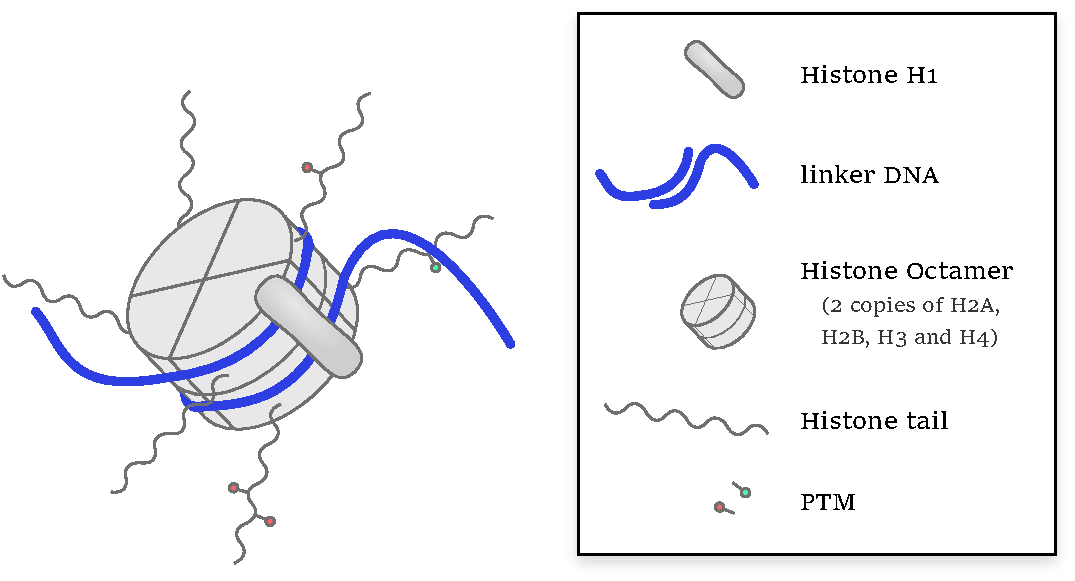
\includegraphics[width=0.7\textwidth]{annotated_nucleosome.pdf}
            \caption{Schematic model of a eukaryotic nucleosome. It consists of DNA wrapped around a histone octamer. The histones themselves are organized as one tetramer (two H3, two H4) and 2 homologous dimers (H2A, H2B). The DNA is kept in place by histone H1, which also plays a role in establishing higher order chromatin structures.}
            \label{img:nucleosome}
        \end{figure}
        %

        %
        Histones contain a great amount of the positively charged amino acids arginine (Arg, R) and lysine (Lys, K), which results in attracting the negatively charged DNA (phosphate backbone) \cite{berg2015stryer}.
        %

        %
        In Eukaryotic nucleosomes, the N-terminal amino acid tails stick out from the histone core complex (see model in fig. \ref{img:nucleosome}) and interact with tails from other nucleosomes and histone 1 (H1) (see fig. \ref{img:nucleosome}) to form higher-order chromatin structures which has a direct influence on transcriptional activity \cite{prohaska2010innovation}. The DNA's local availability as a protein binding site through these higher order structures is often expressed with the terms of open (or active) and closed (or silent) chromatin. However, given that, for instance, transcription factors (TFs) are able to open chromatin \cite{lomvardas2002opening}, it is important to point out the difference between the availability of chromatin and gene transcription activity. Nevertheless, ChAPs play an important role in a general gene activity machinery which is then, in most organisms, followed by more specific mechanisms as, for example, regulation through DNA-sequence-specific TF binding.
        %
    %
    %
    \section{Chemical histone modification}
        \label{subsec:HME}
        %
        Transcriptional regulation can mainly be achieved through two mechanisms \cite{prohaska2010innovation}: firstly by exchanging of ChAP variants \cite{henikoff2008nucleosome} and secondly by chemically modifying ChAPs.
        %


        %
        This thesis is based on one aspect of gene transcription regulation through chromatin (de)stabilization, namely the chemical modification by means of histone-modifying enzyme (HME) complexes. These complexes are able to covalently add or remove chemical groups on amino acids (mostly R and K) at very specific positions on the histone tail. These post-translational modifications (PTMs) are named according to the amino acid they have been bound to. H3K27ac, for instance, denotes an acetylation (\ac/) on lysine 27 (K27) of histone 3 (H3).
        %

        %
        Chemical ChAP modification was mainly observed in Archaea and Eukarya. In Archaea, chemical modification primarily serves the purpose of thermodynamically altering the chromatin's local stability \cite{henikoff2008nucleosome}.
        %

        %
        The presence of these chemical groups changes the charge or polarity of the modified amino acids and thus influences the histone's affinity to the DNA. Histone-acetyl\-transfer\-ases (HATs), for instance, add an acetyl group to lysine, thus neutralizing the positive charge on the ammonium cation at neutral pH (see figure \ref{img:acetyllysineReaction}). This neutralization decreases the attraction to the negatively charged DNA backbone significantly resulting in a more mobile nucleosome and, thus, more active chromatin \cite{berg2015stryer}.
        %

        %
        In Eukaryotes, additionally to the thermodynamic effect, modified histones can also be directly disassembled or evicted resulting in local histone depletion and more open chromatin \cite{henikoff2008nucleosome}.\\
        %

        %
        \begin{figure}[htpb]
            \centering
            \vspace{.5cm}
            \schemestart
                \arrow{0}[,0]
                \chemname{\chemfig{!{lysine}}}{Lysine}\+\chemname{\chemfig{!{acetylcoa}}}{Acetyl-CoA}
                \arrow[-90]
                \chemfig{!{acetyllysine}}\+\chemfig{CoA-SH}\+\chemfig{H^+}
            \schemestop
            \vspace{.5cm}
            \caption{Acetylation of lysine. This reaction is catalysed by the HAT enzyme which by means of the cofactor acetyl coenzyme A (Acetyl-CoA) is able to trigger the transfer (nucleophilic substitution reaction in chemical terms) of an acetyl group onto the nitrogen atom in the side chain of lysine. The latter can be part of a histone tail.}
            \label{img:acetyllysineReaction}
        \end{figure}
        %

        %
        Apart from the acetyl group, a multitude of other markers have been found on histone tails, e.g. methylation (one-, two and three-fold), phosphorylation, ubiquitylation and so forth \cite{bannister2011regulation}. These groups can entail gene transcription activation, silencing (repressing), or fulfil completely different purposes \cite{rossetto2012histone,wang2006histone}. For instance, phosphorylation cascades serve the purpose of rapidly responding to a potential health risk like heat shock \cite{prohaska2010innovation}. Mass-ubiquitination is thought to serve as markers in response to DNA damage resulting in its subsequent repair \cite{zhou2009histone}.\\
        %

        %
        The enzymes' modification activities are not forcibly isolated processes. The different enzyme types as well as the modifications on specific amino acids on the histone tails are connected through complex interaction networks \cite{zhang2015interplay, musselman2012perceiving, ge2019nucleation}. Such crosstalk between different modifications is achieved by the enzymes' ability to “read” modifications and “write” another one, if the reading process was successful. Reading is achieved by binding to specific modifications on the histone tail. A very popular example for such behaviour are enzymes presenting a bromodomain, which specifically binds acetylated lysines \cite{zeng2002bromodomain}. Upon successful binding, the enzyme can then catalyse the covalent modification of an unmodified amino acid. Additionally, proteins can also contain two bromodomains, thus reading two acetylation marks on two different nucleosomes which are arranged in a very specific topology to one another \cite{prohaska2010innovation}.
        %
    %
    %
    \section{Bivalency}
        %
        \label{sec:TheoryBivalency}
        In pluripotent stem cells, nucleosomes have been found to contain both activating and silencing markers on histone tails of one and the same octamer. This bivalent state is believed to maintain a “poised state”, being ready to induce a gene expression cascade as soon as the silencing marker is removed \cite{lesch2014poised,bernhart2016changes}.
        Others believe that this bivalent state is connected to cell division and the ability of inheriting the active gene set for one daughter cell to induce differentiation while the other daughter cell remains a pluripotent stem cell \cite{schuettengruber2017genome}.
        %

        %
        However, the notion of bivalency is not always reduced to one same nucleosome. It was also found that chromatin areas spanning over multiple nucleosomes showed presence of marks that are associated with gene transciption activation as well as silencing without the need of both modification types on one same nucleosome (see review \cite{Hoffmann2015BivalencyReview} for multiple examples). In proximity to genetic domains encoding developmental transcription factors, these poised areas are believed to function as \textit{epigenetic switches}, meaning that, once tilted in the “ON” or “OFF” direction, cell type specific gene activation or silencing can be heritably fixed \cite{Hoffmann2015BivalencyReview}. Thus, it can be argued that bivalent domains serve the purpose of reducing overall transcriptional noise \cite{Bernstein2006BivalentESC} while still keeping a certain degree of transcription willingness of the proximal gene.
        %
    %
    %
%
%
\chapter{Theoretical Background}
\label{cha:theoreticalBackground}
    %
    %

    %
    \section{Chemical master equation}
        \label{subsec:CME}
        %
        %
        The chemical master equation (CME) (see \ref{eqn:CME}, taken from \cite{johnson2021quantifying}) takes the discrete and stochastic nature of a (bio)chemical system into account. It describes the time-dependent evolution of a homogenous system's change in state based on reaction probabilities \cite{Ge2013, johnson2021quantifying}.

        \begin{equation}
            \frac{dP(N,t)}{dt} = \sum^{R}_{r}{\alpha_r (N -\nu_r) \times P(N-\nu_r, t)} - \sum^{R}_{r}{\alpha_r(N) \times P(N,t)}
            \label{eqn:CME}
        \end{equation}

        %
        The CME consists of coupled ordinary differential equations and describes the time $t$ dependent probability $P$ to occupy one state $P(N,t)$ of a discrete set of states. $N$ is a composition vector describing the abundance of each chemical species. $R$ denotes the number of all possible reactions $r$. $\nu_r$ is the stoichiometric vector that thus describes the change of the number of every chemical species in $N$ if the system undergoes reaction $r$. $\alpha_r$ indicates the probability per unit time that $r$ can occur.
        %

        %
        Analytical solutions of the CME are rarely used in practical models, especially in biological systems \cite{johnson2021quantifying} because of the high computational complexity in real-life inspired models, as solving the CME scales exponentially with the number of different chemical entities in the system.
    %
    %
    \section{Dynamic histone PTM models}
        %

        %
        In order to establish the CME for a histone PTM model, one can establish the modification concentration dependent differential equation \cite{lemons1908paper} for each modification type with respect to the HME types that take part in changing the respective modification concentration.
        %

        %
        For practical illustration, consider a histone PTM model which includes two mutually-exclusive modifications: acetylation (\ac/) and methylation (\me/) of nucleosomes. The nucleosomes are not distinguishable from one another apart from being either acetylated, methylated or unmodified. The HMEs contained in the system are \ac/ writers, \ac/ removers, \me/ writers and \me/ removers.
        %

        %
        The CME for such a system was already formed and analysed by Mayer in \cite{mayer2020langevin}.
        %

        %
        Eqns. \ref{eqn:noncooperative} describe the CME for $a = \frac{A}{N}$ and $m = \frac{M}{N}$ with $A$ the number of acetylated nucleosomes, $M$ the number of methylated nucleosomes and $N$ the total number of nucleosomes. $\alpha_i$ and $\beta_i$ are probability coefficients taking into account the types, association and dissociation rates of the enzymes in the system.
        %

        %
        \begin{subequations}
            \begin{align}
                &\frac{\partial a}{\partial t} = \underbrace{- \alpha_1 a }_{\textrm{ac removal}} + \underbrace{ \alpha_2 a (1-a-m) }_{\textrm{ac addition}}\\
                &\frac{\partial m}{\partial t} = \underbrace{- \beta_1 m }_{\textrm{me removal}} + \underbrace{ \beta_2 m (1-a-m) }_{\textrm{me addition}}
            \end{align}
            \label{eqn:noncooperative}
        \end{subequations}
        %

        %
        It is important to note that $a$ and $m$ describe the relative number of the corresponding modification among the nucleosomes which implies that every nucleosome with a specific type of modification is one chemical species. If one considers a system in which nucleosomes have one and the same neighbour the entire time one could define enzymatic reactions that take these fixed neighbour relations into account.
        %

        %
        An appropriate CME model would then require to establish and solve the CME for every nucleosome while the CME for nucleosome $i$ would depend on the number of next-neighbours equal to the biggest enzyme reading frame in the system. For instance, if the enzyme only considers the next neighbours $i+1$ and $i-1$ of the nucleosome $i$ to be modified, the CME system would change to eqns. \ref{eqn:neighbourDependent}.
        %

        %
        \begin{subequations}
            \begin{align}
                &\frac{\partial a_i}{\partial t} = - \alpha_1 (a_{i-1} + a_i + a_{i+1}) + \alpha_2 (a_{i-1} + a_i + a_{i+1}) \times (1-a-m)\\
                &\frac{\partial m_i}{\partial t} = - \beta_1 (m_{i-1} + m_i + m_{i+1}) + \beta_2 (m_{i-1} + m_i + m_{i+1}) \times (1-a-m)
            \end{align}
            \label{eqn:neighbourDependent}
        \end{subequations}
        %

        %
        This differential equation system quickly increases in complexity and dimensionality with increasing number of nucleosomes in the system and higher reach of the enzymes up to a point where an analytical solution is impossible to achieve. Mainly for this reason, it is convenient to numerically simulate the time-dependent evolution of the system.
        %
        %
    %
    \section{Stochastic simulation algorithm}
    \label{subsec:Gillespie}
        %
        Gillespie's \textit{stochastic simulation algorithm} (SSA) simulates the evolution in time of a spatially homogenous molecular mixture with a discrete number of reactants under specification of the coupled reaction channels based on stochastic chemical kinetics \cite{gillespie1976general, gillespie1992rigorous}. This is useful especially when the practice of solving the chemical master equation analytically is not ideal.
        %

        %
        Gillespie takes an event-based time step approach. This ensures that at every time step, exactly one event is taking place. This approach obviously reduces the overhead compared to an equidistant time step approach (see fig. \ref{img:Gillespie_timeSteps}) and can massively facilitate implementation and later interpretation of the simulation results.
        %

        %
        \begin{figure}[htpb!]
            \centering
            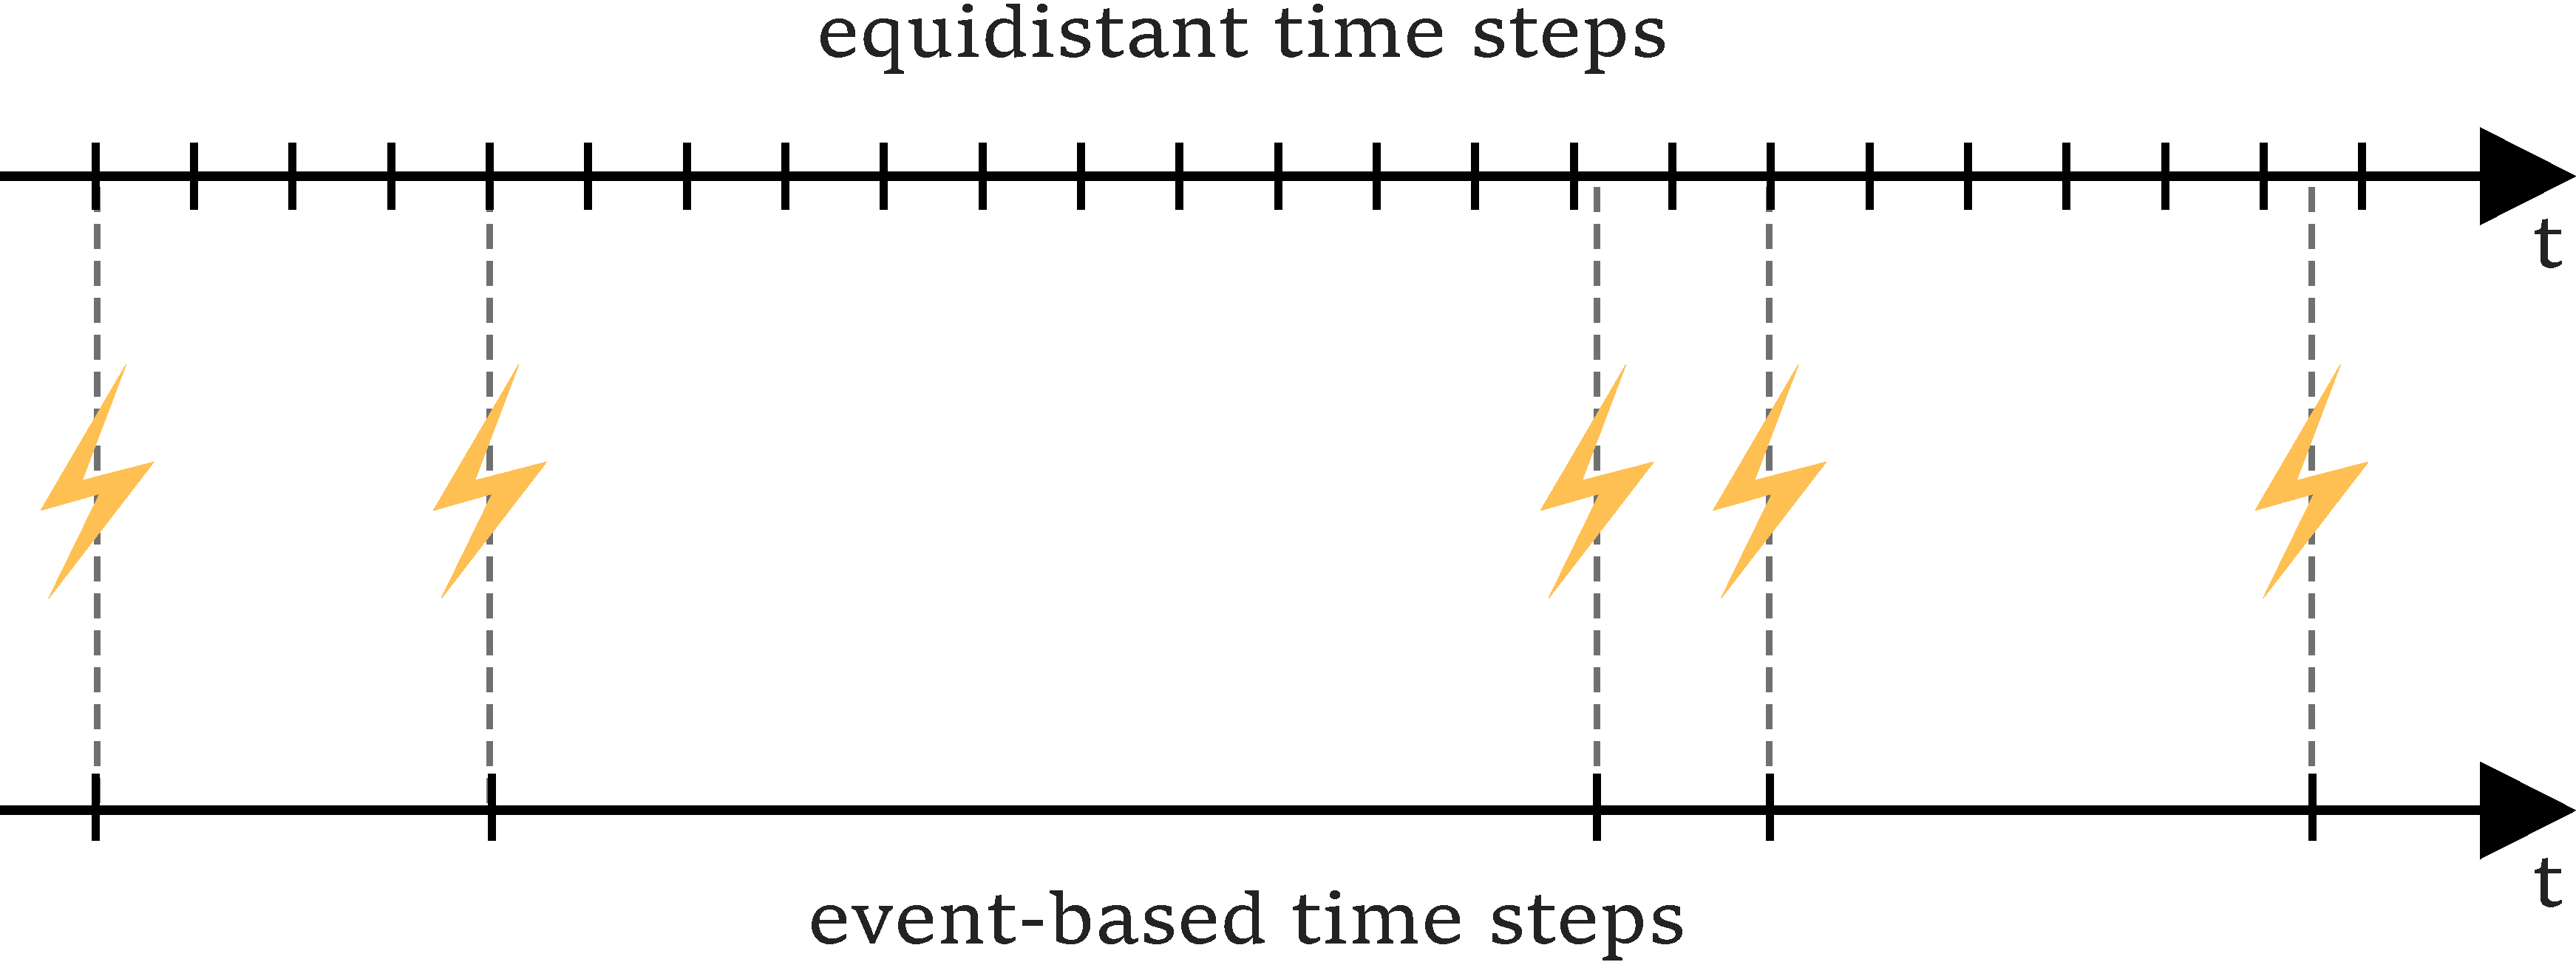
\includegraphics[width=0.7\textwidth]{Gillespie_timeSteps.pdf}
            \caption{Schematic illustration of equidistant time steps vs. event-based time steps inspired by Mayer in \cite{mayer2020langevin}.}
            \label{img:Gillespie_timeSteps}
        \end{figure}
        %

        %
        The algorithm summarizes the probabilities of every reaction $r$ (or reaction channel) defined in the CME and assesses if this reaction is feasible in function of the composition vector $N$. If a chemical species is depleted at a certain time, every reaction containing this reagent will not be taken into account for the choice of the next event. The probabilities of the possible reaction channels are summarized into a propensity sum.
        %

        %
        Then, two numbers are chosen by mapping a uniformly random number on the unit interval to the reaction that contributes the respective propensity to the propensity sum. An event is then chosen based on one random number while the other one determines the time elapsed since the last event. The time in between reactions is Poisson-distributed. In order to be able to use the random number drawn from a uniform distribution, it is transformed via the inversion method.
        %

        %
        The elapsed time depends on the number of possible reactions at every time step. If many events are contributing to the propensity sum at this point in time, the time in between events is smaller. Conversely, if only few events are possible at this time step, the time in between events is larger.\\
        %


        % %
        % In more systematical terms, Gillespie's algorithm can be summarized in the following 4 steps \cite{gillespie1977exact, mayer2020langevin}:
        % %

        % %
        % \begin{itemize}
        %     \item \textbf{Step 0 (initialization):} Set an initial starting state $X$ and a rule set. Set $t = 0$.
        %     \item \textbf{Step 1:} Calculate the propensity sum $a_0$ as the sum of all legal reactions and their occurrence possibility based on their association/dissociation rates and their concentration.
        %     \item \textbf{Step 2:} Based on random numbers, choose a specific reaction channel $\mu$ as the event to happen in this time step as well as the time $\tau$ elapsed from the previous event to the present one.
        %     \item \textbf{Step 3:} Update the time $t_{i+1} = t_i + \tau$ as well as the effect that $\mu$ has on the system $X_{i+1} = \mu (X_i)$. Continue with step 1.
        % \end{itemize}
        % %
    %
    %
    \section{\ed/}
    \label{subsec:EpiDynast}
        %
        The software used in this thesis is \ed/ (\textbf{Epi}genetic \textbf{Dyna}mics \textbf{S}imulation \textbf{T}ool), which bases on \texttt{StoChDyn} by Arnold et al. \cite{arnold2013chromatin} and was developed by N. Herbig et al. (unpublished results).
        %

        %
        \ed/ is a PTM simulation software which, at its core, uses Gillespie's SSA in order to show the dynamic change on a nucleosome string as a function of time.
        %

        %
        The main working mechanism may be outlined as follows: First, one defines the enzyme types contained in the system (see example in \ref{app:rulefile}) and a starting nucleosome state (see example in \ref{app:statefile}), which is defined as an array of nucleosomes reduced to their PTMs. Then, after specifying the overall run time (see example in \ref{app:paramfile}), \ed/ simulates the stochastic time-dependent change of said modifications on the nucleosome array, exactly one event at a time. The two events that can occur for each enzyme are either an association (read) step or a reaction (write) step where the latter immediately entails the enzyme's dissociation from the nucleosome.
        %

        %
        \subsection{Chromatin Model}
        \label{subsec:ChromatinModel}
            %
            Chromatin in \ed/ is modelled as an array of nucleosomes. The nucleosomes hold their respective position on a string so that the neighbour relations are fixed. That way, every nucleosome has exactly two neighbouring nucleosomes (one for  the first and last nucleosome on the string, called border nucleosomes) that stay identical throughout the entirety of a simulation. Furthermore, the nucleosomes are reduced to presence or absence of PTMs on their tails. Every nucleosome can hold zero or more modifications at the same time. DNA is not explicitly included in \ed/'s chromatin model.
            %

            %
            The nucleosome string can either be non-cyclic or cyclic. In the cyclic case, the enzymes can read nucleosomes from the start as well as the end of the string, i.e. both border nucleosomes, simultaneously. In the non-cyclic case, the first and last nucleosome logically only have one neighbour.
            %

            %
            Every simulation is provided a starting state that fixes the number of nucleosomes as well as their modifications at time step $t=0$.
            %
        %

        \subsection{Enzyme model}
            %

            %
            The enzymes in \ed/ are mainly described by their reaction type, the pattern it reads in order to perform the reaction, their association and their dissociation rate. The reaction type defines the change which the enzyme performs on the nucleosomes' modifications. Generally, the enzymes are either modification adders or modification removers.
            %

            %
            % The enzyme's context can be defined as the set of one or more nucleosome PTMs that must be present in a precisely determined neighbour-relation to the nucleosome that is intended to be changed. If the enzyme finds the needed context to be unfitting, the reaction of this enzyme with the determined nucleosome is not taken into the propensity sum of that simulation step (see the explanation of Gillespie's algorithm in \ref{subsec:Gillespie}). Random enzymes have a context which exclusively contains the one nucleosome that is about to be modified by the enzyme (see \ref{subsec:EnzymeTypes} for details). The reaction type and context are defined together by a specific set of (possibly multiple) rules for each enzyme.
            %

            %
            An enzyme's reaction type can be defined by means of a rewriting rule which consists of a pattern of (un)modified nucleosomes read by the enzyme and the modification triggered upon dissociation. The enzyme's pattern includes the nucleosome to be modified as well as the enzyme's context which needs to be found on the string of nucleosomes in order for the enzyme to become active. It is important to note that the neighbour relations between the nucleosomes in the enzyme's pattern are strictly fixed. If, for instance, one wants an unmodified nucleosome  in between the nucleosome to be modified and an acetylated nucleosome, this unmodified nucleosome must be explicitly indicated as part of the context. The enzyme's pattern includes the nucleosome that is modified upon dissociation as well as the precise context around it. It can contain one or multiple nucleosomes.
            %

            %
            As an example, a linear acetylation adder enzyme would look for a pattern with two neighbouring nucleosomes, one acetylated and the other one unmodified, and acetylate the latter.\\
            %

            %
            On a sidenote, given that the pattern indicated in the enzyme rule set is an important aspect of \ed/, an analytical solution of the CME would not be the best approximation. Also, \ed/'s model strongly depends on discrete numbers such as the number of nucleosomes on the string, rendering mere state concentrations without positional information insufficient. Thus, the analytical solution of the CME as a continuous system makes it even more unfitting as an approximation for the system at hand. This is one more reason for performing a numeric simulation of the CME by means of Gillespie's algorithm.\\
            %

            %
            The association and dissociation steps are considered the enzyme's reaction channels by the underlying SSA. The entirety of rewriting rules of all the enzymes in the system are summarized in a rule set file (see \ref{app:rulefile} for an illustrative rule file.)
            %

            %
            The association rate together with the enzyme's concentration define the enzyme's affinity to its substrate. The dissociation rate in turn defines the enzyme's speed concerning reaction and diffusion away from the modified nucleosome.
            %

            %
            On a sidenote, Gillespie's algorithm and thus \ed/ offer the possibility to model concentration depletion effects.\\
            %


            In order to clarify the meaning of the vocabulary concerning the enzyme models, consider the following illustration:
            %

            %
            For the HAT enzyme mentioned earlier, one would define the enzyme’s pattern as an unmodified nucleosome, as this is needed in order for the enzyme to perform its specific chemical modification reaction on the nucleosome string, which is acetylation of an unmodified nucleosome. Possibly, the enzyme needs a specific reading pattern in order to bind to the string in proximity of the nucleosome to be modified. This is the case when concerning self-reinforcing enzymes, for instance, which read their own modification and are then able to write it to another unmodified nucleosome which results in a positive feedback loop (see bromodomain mentionned earlier). Such specific reading/binding patterns are also contained in the context of this specific enzyme.
            %

            %
            Thus, in summary, the enzyme in a rule set pattern is a summary of rules that impose constraints on the presence or absence of modifications on the nucleosome string in order for the enzyme to gain reading (and subsequent writing) ability.\\
            %
        %
        %
    %

    %
    %
    \section{Previous work}
        %

        %
        In \cite{mayer2020langevin}, Mayer analysed dynamic histone PTM models concerning the stability of a system containing acetylation and monomethylation and built a mathematical foundation based on previous work from Sneppen \cite{sneppen2014models}.
        %

        %
        Each HME type induces an individual stability trend among the configurations which results in a vector field specific to each type of enzyme. In more complex systems with a multitude of different enzyme types, these vector fields are combined by superposition and create a resulting vector field containing zero or more fix points, depending on the un-, mono- or multistable nature of the system.
        %

        %
        %
        \subsection{Monostable states}
            \label{subsec:monostability}
            %
            In \cite{mayer2020langevin}, Mayer analysed eqns. \ref{eqn:noncooperative} that originate from \cite{sneppen2014models} and describe a histone PTM model in which nucleosomes adopt one out of three mutually-exclusive states: unmodified (\textit{un}), acetylation (\ac/) and methylation (\me/). The nucleosomes are not differentiatable from one another apart from being either acetylated, methylated or unmodified. The HME contained in the system are \ac/ writers, \ac/ removers, \me/ writers and \me/ removers.
            %

            %
            4 critical values were found in the Cartesian coordinate system $(m,a)$ with origin $(0,0)$, $m$ the amount of methylated nucleosomes and $a$ the amount of acetylated nucleosomes. Three are fix points at $(0,0)$, $(0,1-\nicefrac{\beta_1}{\beta_2})$, $(1-\nicefrac{\alpha_1}{\alpha_2},0)$ and one is a separatrix whose gradient depends on the ratio between $\nicefrac{\alpha_1}{\alpha_2}$ and $\nicefrac{\beta_1}{\beta_2}$ and which connects the two non-trivial fix points. The separatrix always has a gradient towards one of the non-trivial fix points, except for the case $\nicefrac{\alpha_1}{\alpha_2} = \nicefrac{\beta_1}{\beta_2}$. Here, the separatrix has no gradient (see fig. \ref{img:nonCooperativeVectorFields} \textbf{(b)}).
            %

            %
            \begin{figure}[!htbp]
                \centering
                \begin{minipage}{0.3\textwidth}
                    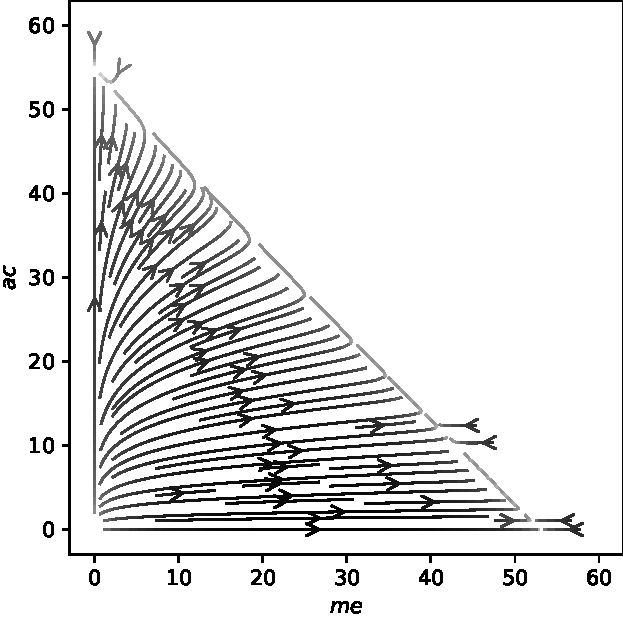
\includegraphics[width=\textwidth]{vectorfield_noncooperative_assymetric_monostable_ac.pdf}
                    \caption*{\small \textbf{(a)}}
                \end{minipage}
                \begin{minipage}{0.3\textwidth}
                    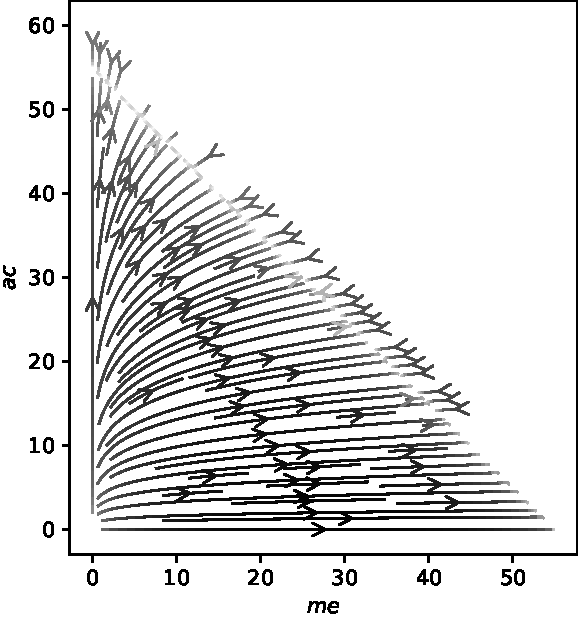
\includegraphics[width=\textwidth]{vectorfield_noncooperative_asymmetric_multistable.pdf}
                    \caption*{\small \textbf{(b)}}
                \end{minipage}
                \begin{minipage}{0.3\textwidth}
                    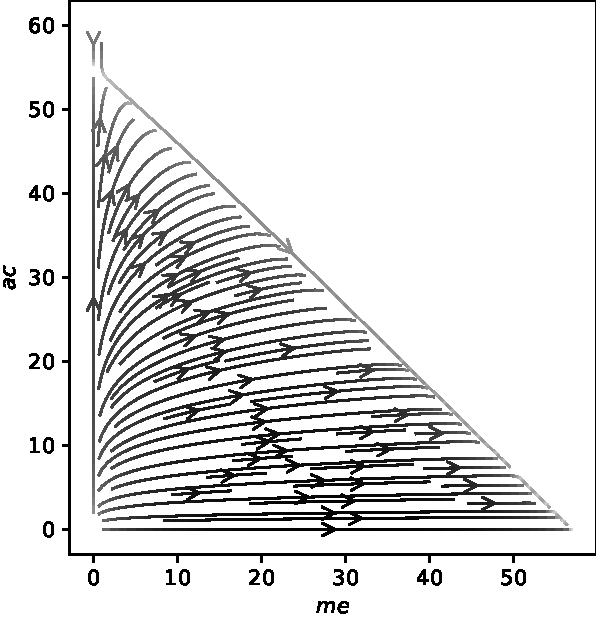
\includegraphics[width=\textwidth]{vectorfield_noncooperative_assymetric_monostable_me.pdf}
                    \caption*{\small \textbf{(c)}}
                \end{minipage}
               \caption{Vector fields describing the non-cooperative 60 nucleosome system with varying enzyme rates. These mainly define the parameters $\alpha_n$ and $\beta_n$ if the enzyme types are constant. The axes describe in absolute numbers the occurrence of methylation (x-axis) and acetylation (y-axis). \textbf{(a)} describes the case for $\nicefrac{\alpha_1}{\alpha_2} > \nicefrac{\beta_1}{\beta_2}$ resulting in a separatrix with gradient towards $(0,N(1-\nicefrac{\beta_1}{\beta_2}))$. In \textbf{(b)}, the equality $\nicefrac{\alpha_1}{\alpha_2} = \nicefrac{\beta_1}{\beta_2}$ results in a zero-gradient separatrix. In \textbf{(c)}, $\nicefrac{\alpha_1}{\alpha_2} < \nicefrac{\beta_1}{\beta_2}$ results in a separatrix with gradient towards $(N(1-\nicefrac{\alpha_1}{\alpha_2}),0)$. From Mayer in \cite{mayer2020langevin}.}
               \label{img:nonCooperativeVectorFields}
            \end{figure}
            %

            %
            One could argue, that for the case of $\nicefrac{\alpha_1}{\alpha_2} = \nicefrac{\beta_1}{\beta_2}$, the zero-gradient separatrix interpreted as a set of points fulfilling a linear equation presents an infinite amount of stable points, thus rendering this specific system multistable. However, one point on the separatrix can hardly be described stable, because it is not resistant to small perturbations. In fact, even the most atomic displacement, namely the state change of one nucleosome, most likely leads to another point on the separatrix and not forcibly to the previous one. Thus, the separatrix as a whole, containing both non-trivial fix points can be described as stable and disqualifies every other point on the separatrix from individual stability in the case of $\nicefrac{\alpha_1}{\alpha_2} = \nicefrac{\beta_1}{\beta_2}$, hence the monostable nature of all the systems in fig. \ref{img:nonCooperativeVectorFields}.
            %


        \subsection{Bi- and multistable states}
            \label{subsec:multistable}
            %
            In order for a dynamic histone PTM system to be bistable, the enzymes have to show cooperativity \cite{dodd2011barriers,sneppen2019theoretical,mayer2020langevin}. According to Sneppen \cite[][p.48]{sneppen2014models}, \enquote{cooperative binding means that the probability of occupying a state increases more than linearly with the concentrations of the binding molecules}.
            %

            %
            In \cite{dodd2011barriers}, Dodd et al. specify the nature of cooperativity in order to reach ultrasensitivity\footnote{From Dodd et al. \cite{dodd2011barriers}: \enquote{Ultrasensitivity is a nonlinearity that magnifies any numerical advantage of one nucleosome type over another, allowing positive feedback to strongly push the system away from intermediate states and towards a large majority of one or other type.}} and thus a robustly bistable system as follows\footnote{citations inside the quote changed their appearance in order to remain functional and to stylistically fit this work}:
            %

            %
            \begin{quote}
                “Cooperativity can be direct, where two modified nucleosomes act together to recruit an enzyme to modify a third nucleosome \cite{3dodd2007theoretical,11sedighi2007epigenetic,15micheelsen2010theory}, or indirect, where each modified nucleosome catalyzes one of two separate modification reactions to fully convert a third nucleosome \cite{3dodd2007theoretical,13david2009inheritance}. A critical requirement for ultrasensitivity is that modified nucleosomes must act nonlocally, stimulating modification of nucleosomes located some distance away on the DNA. This long-range interaction is necessary for any nucleosome to be able to ‘sense’ the majority nucleosome type within the patch and cannot be provided by simple neighbor-to-neighbor contact \cite{3dodd2007theoretical,15micheelsen2010theory}.”
            \end{quote}
            %

            %
            Thus, for single enzymes, direct cooperativity can only be a property of those enzymes which read at least three nucleosomes. Indirect cooperativity can be achieved in a two-step process which involves two enzymes that each read at least two nucleosomes.
            %

            %
            In order to reach robust bistability, the “read-only” nucleosomes should not be direct neighbours of the nucleosome to be (un)modified, as is the case in Dodd et al.'s model where every nucleosome is able to "see" each other one, which they justify by biological phenomena such as higher order chromatin structure or DNA looping \cite{dodd2007theoretical}. This non-local interaction allows the modification that is superiorly prevalent over the whole string at that moment to be accounted for and recognized by the enzymes.
            %

            %
            It is important to stress that cooperativity is not imperatively necessary in order for a system to be bistable \cite{dodd2007theoretical}. However, according to Dodd et al., the absence of cooperativity makes bistability hard to achieve, hardly robust and only possible under conditions, where there are very low noise levels within the system.
            %

            %
            On a sidenote, the definition of cooperativity given by Dodd et al. might seem slightly counterintuitive from a biochemical point of view, where the notion of cooperativity is strongly associated to be an asset of the enzyme \cite{cooperativityDefBritannica}. In contrast, according to Dodd et al., cooperativity is described as a property of a set of nucleosomes being able to “cooperate” in order to recruit an enzyme and catalyse a reaction. A biochemist might be more comfortable with the enzymes being the active part in the system and most notably the catalyst of the occurring reactions instead of the nucleosomes, which most definitely do not catalyse any chemical reaction. As a consequence, in this work, direct cooperativity will be defined as a property of cooperative enzymes whereas indirect cooperativity involves a set of two non-cooperative enzymes.
            %

            %
            Even though the biochemical implications were not ideally put, the mathematical implications explained by Dodd et al. are untouched from these imprecisions.\\
            %

            %
            Mayer in \cite{mayer2020langevin} expressed the time dependent concentration of the modifications on the nucleosome string with cooperative modification adders and non-cooperative modification removers in the CME system depicted in eqns. \ref{eqn:cooperative}.
            %

            %
            \begin{subequations}
                \begin{align}
                    &\frac{\partial a}{\partial t} = \underbrace{- \alpha_1 a }_{\textrm{ac removal}} + \underbrace{ \alpha_2 N^2 a^2 (1-a-m) }_{\textrm{ac addition (cooperative)}}\\
                    &\frac{\partial m}{\partial t} = \underbrace{- \beta_1 m }_{\textrm{me removal}} + \underbrace{ \beta_2 N^2 m^2 (1-a-m) }_{\textrm{me addition (cooperative)}}
                \end{align}
                \label{eqn:cooperative}
            \end{subequations}
            %

            %
            This cooperative system is now cubic in both dimensions and exhibits thus up to 9 critical points. Some of these can quite easily be identified graphically.
            %

            %
            Fig. \ref{img:cooperativeVectorField} depicts the vector field of a system with random and cooperative enzymes at symmetrical rates for methylation and acetylation. Some critical values can clearly be identified. They are summarized in tab. \ref{tab:cooperativeCriticalValues}.
            %

            %
            \begin{figure}[htbp!]
                \centering
                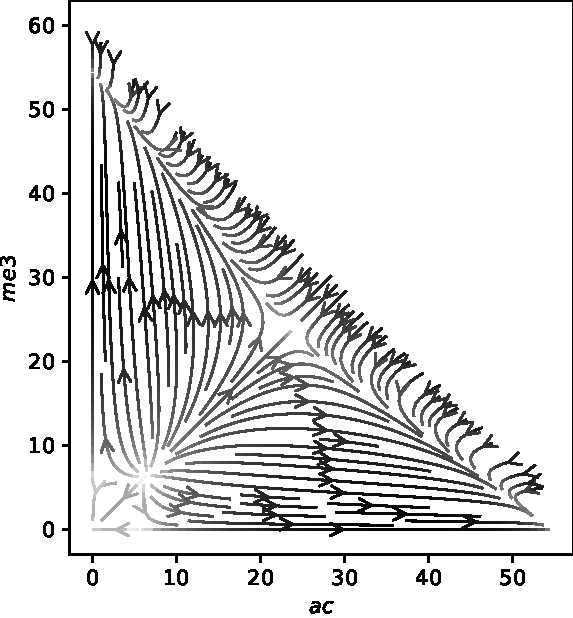
\includegraphics[width=.5\textwidth]{vectorfield_cooperative.pdf}
                \caption{Vector fields describing the cooperative 60 nucleosome system with varying enzyme rates. These mainly define the parameters $\alpha_n$ and $\beta_n$ if the enzyme types are constant. The axes describe in absolute numbers the occurrence of acetylation (x-axis) and methylation (y-axis). From \cite{mayer2020langevin}.}
                \label{img:cooperativeVectorField}
            \end{figure}
            %

            %
            \begin{table}[htbp!]
                \caption{Critical values in $(a,m)$ notation as identified graphically in fig. \ref{img:cooperativeVectorField}.}
                \begin{center}
                    \begin{tabular}{l r}
                        \hline
                        \textbf{critical point} & \textbf{stability} \\
                        \hline
                        $(0,0)$     & stable \\
                        $(8,8)$     & unstable \\
                        $(0,5)$     & unstable \\
                        $(5,0)$     & unstable \\
                        $(0,55)$    & stable \\
                        $(55,0)$    & stable \\
                        $(25,25)$   & saddle point \\
                        \hline
                    \end{tabular}
                \end{center}
                \label{tab:cooperativeCriticalValues}
            \end{table}
            %
        %
        %
        \subsection{Bistable switching}
        \label{sec:TheoBistableSwitching}
        %

        %
        In the context of multistable histone PTM systems, the term of epigenetic switches (explained in \ref{sec:TheoryBivalency}) might become ambiguous.
        %

        %
        On the one hand, as explained before, an epigenetic switch linked to bivalency might describe a three state mechanism: the aforementioned irreversible “ON” and “OFF” states, but also the poised “STANDBY” state \cite{Hoffmann2015BivalencyReview}.
        %

        %
        On the other hand, epigenetic switches might be understood following the analogy of a light switch with the “ON” and “OFF” states being the only possible stable states without any relation to bivalent chromatin at all. A possible application of such a system in the context of evolution has been theoretically discussed in \cite{gomez2019epigenetic}. Given that epimutations (i.e. switching from one stable state to the other) is usually much faster than genetic mutation, the phenotypic diversity and quick adaptation might be an evolutionary advantage in fast fluctuating environments.\\
        %

        %
        Both concepts are relevant to this work. Accordingly, \textit{bistable switching} is hereby explicitly defined as the possibly reversible change from one stable activating or silencing macrostate to the respective other one in absence of an intermediate identifiable “STANDBY” state.
        %

        %
        In contrast, \textit{bivalent switching} is hereby defined as the transition from a pseudostable intermediate (“STANDBY”) state to a stable activating or silencing macrostate within a histone PTM system. Contrarily to the corresponding concept in \cite{Hoffmann2015BivalencyReview}, bivalent switching as defined in the scope of this work is not forcibly irreversible, making bivalent switching more relatable to the given definition of bistable switching.
        %
        %
    %
    %
    %
    %
    \section{Impact of this work}
        %
        Although the mathematical foundation on whether a system can and cannot show bistability was already established, the execution in terms of building a model and rigorously identifying the influence of different factors within the model on the dynamics of a bistable system have, to the knowledge of the author, not been explored yet.
        %

        %
        Also, to date, bistable systems have not yet been modelled by means of a software that takes limited enzyme reach into account, while still allowing non-local interactions, like \ed/ does. This is an important distinction from other models, because neighbour-to-neighbour relations are not neglected, which marks an important step towards real-life chromatin systems.\\
        %

        %
        This thesis will show the potential and limitations of a model with fixed neighbour relations concerning bistability and the switching between stable states throughout the simulation. Furthermore, this work will take a deep look at the working mechanisms of bistability occurring on non-cyclic, as well as cyclic nucleosome strings.
        %
    %
    %
%
%

\chapter{Methods}
    \label{cha:methods}
    %

    %
    \section{Chromatin Specifications}
        \label{sec:ChromatinModel}

        %
        The chromatin model in this work can be reduced, so that a nucleosome is modelled as one single amino acid (e.g. $K27$) which can be either acetylated (referred to as active) or monomethylated (referred to as silenced). Di- and trimethylation will not be featured in this work.
        %

        %
        The nucleosome string is either modelled to be non-cyclic (as done in \ref{sec:ResNon-cooperative} and \ref{sec:ResNonCyc}) or cyclic (\ref{sec:ResBistableSwitching} to \ref{sec:ResBoundariesBistability}). In the cyclic case, the enzymes' pattern can include nucleosomes from the start as well as the end of the string simultaneously. In the non-cyclic case, the first and last nucleosome logically only have one neighbour.
        %

        %
        The non-cyclic models contain 60 nucleosomes whereas the cyclic ones only contain 40 nucleosomes in order to reduce computation time and storage space.
        %

        %
        The starting state for every simulation in this work is a completely unmodified nucleosome string. As long as there are random adders in the system (which is the case for every system featured in this work), the completely unmodified string logically is an unstable configuration which does not offer any sort of bias in the direction of acetylation or methylation respectively, hence the choice of an entirely unmodified starting state. The time it takes for the system to adjust in order to establish a fully modified string is negligible compared to the total time of one simulation run.
        %
    %
    %
    \section{Enzyme specifications}
    \label{sec:EnzymeTypes}
        %

        %
        All enzyme adder rules exclusively work on an unmodified nucleosome. Accordingly, for instance, a methylated nucleosome must be demodified first before an \ac/ adder enzyme can acetylate it. The opposite counts for an acetylated nucleosome. In summary, the modification pathway $ac \longleftrightarrow un \longleftrightarrow  me$ is imperative for all enzyme rules.
        %

        %
        The enzyme rule sets as well as their rates were defined symmetrically throughout the entirety of the simulations that were done for this work. Thus, for instance, every rule which defines the addition of an acetyl group to a nucleosome next to one that already has an acetyl group is defined in either direction on the string and has a methylation counterpart at equal association and dissociation rates.
        %

        %
        One of the strengths of Gillespie's algorithm is the possibility of emulating a system where molecule concentrations are very low, to the extent that they deplete over time. To that effect, the association rate (not the dissociation rate) set in the enzyme rule set is normally multiplied by the given concentration in the conventional SSA. Concentration depletion effects provided as a feature by \ed/ were not used in this work. Accordingly, all enzymes were assumed to be equally and infinitely available in the simulation. Supposing that there are more enzymes of one type in the system than could ever bind onto the string simultaneously, this seems to be an appropriate approximation. As a result, the concentration is supposed to be 1 for each enzyme rendering the assciation rates and dissociation rates directly comparable to each other.
        %

        %
        A short summary of all enzyme types featured in this work can be found in tab. \ref{img:enzymeTypeSummary}.
        %

        %
        \subsection{Enzyme types}

            %
            \subsubsection{Linear modifier enzymes}
                %

                %
                Linear modifier enzymes are used to extending sites which contain a specific modification (e.g. acetylation, see fig. \ref{img:linearEnzymes}) by either propagating said modification from nucleosome to neighbouring unmodified nucleosome (fig. \ref{img:linearEnzymes} \textbf{(a)}) or by deleting an opposing modification next to a nucleosome with the desired one (fig. \ref{img:linearEnzymes} \textbf{(b)}). They always have direct neighbour reach.
                %

                %
                \begin{figure}[htpb!]
                    \centering
                    \begin{minipage}[t][5cm]{\textwidth}
                        \begin{minipage}{0.15\textwidth}
                            \caption*{\small \textbf{(a)}}
                        \end{minipage}
                        \begin{minipage}{0.8\textwidth}
                            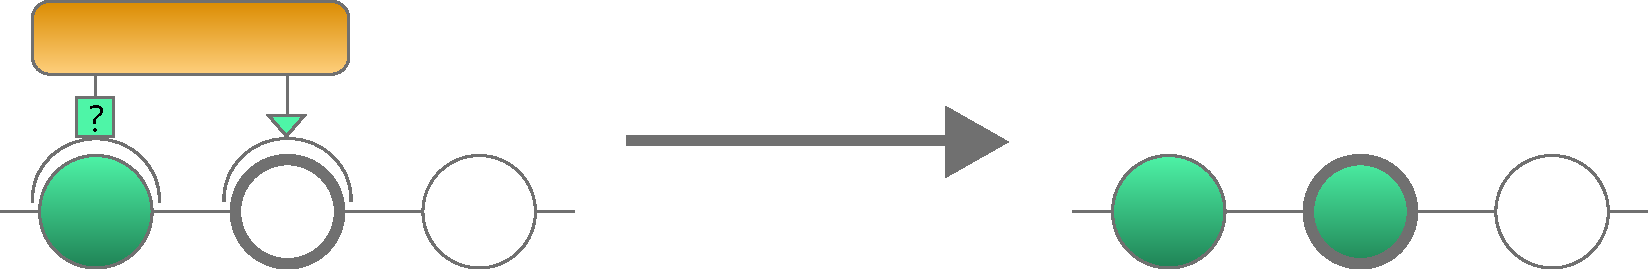
\includegraphics[width=\textwidth]{enzymes/linear_a.pdf}
                        \end{minipage}
                        \vfill
                        \begin{minipage}{0.15\textwidth}
                            \caption*{\small \textbf{(b)}}
                        \end{minipage}
                        \begin{minipage}{0.8\textwidth}
                            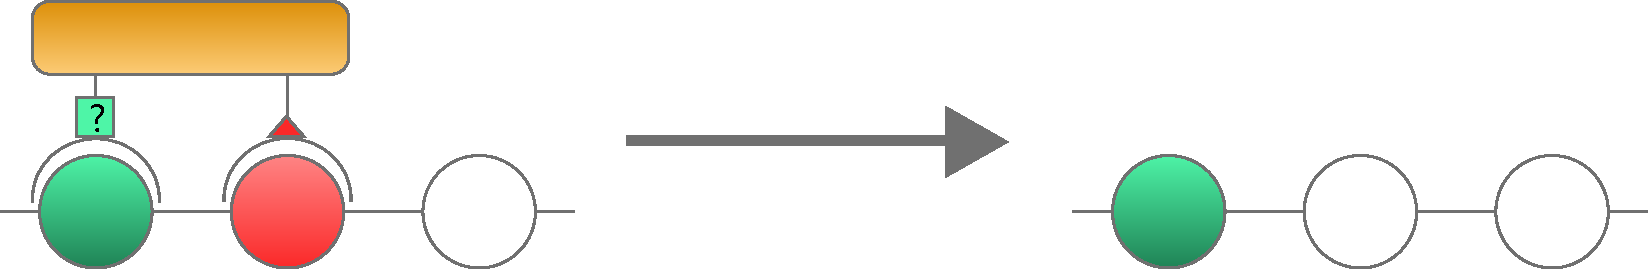
\includegraphics[width=\textwidth]{enzymes/linear_b.pdf}
                        \end{minipage}
                    \end{minipage}
                    \caption{Simplified model of linear modifier enzyme \textbf{(a)} acetylation addition and \textbf{(b)} methylation removal reactions. Acetylated nucleosomes are coloured in green, methylated nucleosomes are red and colourless ones are unmodified. The reactions shown are also defined in the rule set to occur in the opposite direction. Linear modifier enzymes in favour of methylation extension (or acetylation deletion) work analogically.}
                    \label{img:linearEnzymes}
                \end{figure}
                %
            %
            %
            \subsubsection{Cooperative modifier enzymes}
                \label{subsubsec:coopEnzymes}
                %

                %
                \begin{figure}[htpb!]
                    \centering
                    \begin{minipage}[t][3cm]{\textwidth}
                        \begin{minipage}{0.15\textwidth}
                            \caption*{\small \textbf{(a)}}
                        \end{minipage}
                        \begin{minipage}{0.8\textwidth}
                            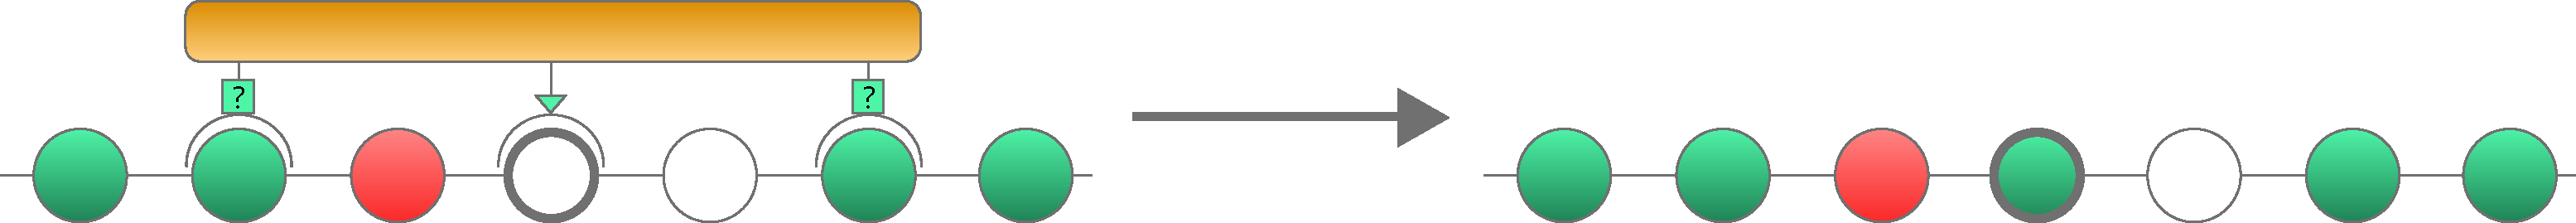
\includegraphics[width=\textwidth]{enzymes/coop_a.pdf}
                        \end{minipage}
                    \vfill
                        \begin{minipage}{0.15\textwidth}
                            \caption*{\small \textbf{(b)}}
                        \end{minipage}
                        \begin{minipage}{0.8\textwidth}
                            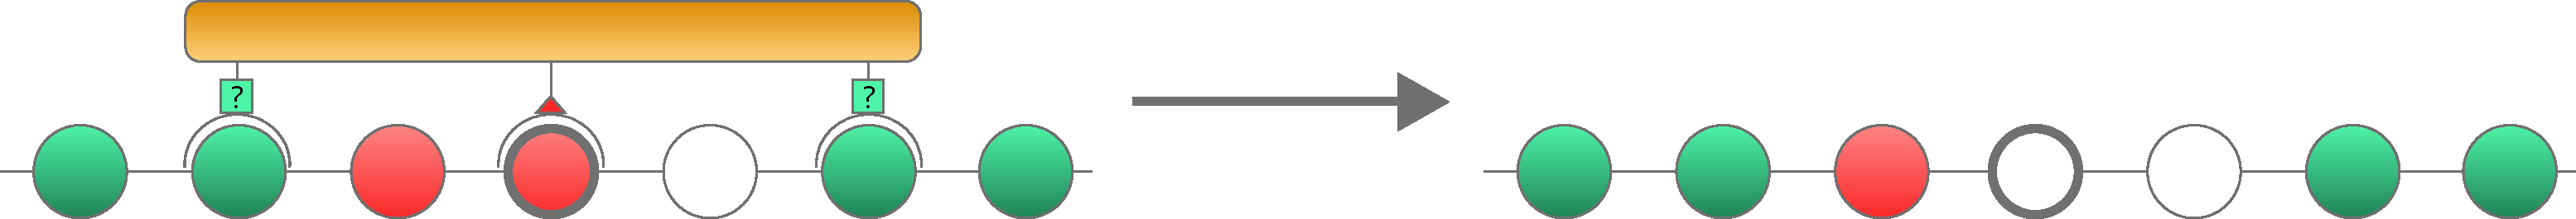
\includegraphics[width=\textwidth]{enzymes/coop_b.pdf}
                        \end{minipage}
                    \end{minipage}
                    \caption{Simplified model of cooperative modifier enzyme \textbf{(a)} acetylation addition and \textbf{(b)} methylation removal reactions. Acetylated nucleosomes are coloured in green, methylated nucleosomes are red and colourless ones are unmodified. The reactions shown are also defined in the rule set to occur in the opposite direction. Cooperative modifier enzyme methylation addition and acetylation removal work analogically.}
                    \label{img:coopEnzymes}
                \end{figure}
                %

                %
                Cooperative modifier enzymes generally read the state of two different nucleosomes on the string and write to or remove a modification from a third nucleosome. It is important to note that the two nucleosomes that are read do not need to have next-neighbour relation to the one the enzyme is modifying.  Thus, to some extent, these enzymes, unlike any other enzyme featured in this work, take the global modification trend on the string into account: if many nucleosomes are acetylated, then cooperative modifier enzymes in favour of acetylation (meaning cooperative acetylation adders and cooperative methylation removers) are more active which, in turn, reinforces the acetylation distribution on the string.
                %

                %
                The cooperative modifier enzymes in this work are implemented in a way that they are always reading two nucleosomes that are equally far away from the nucleosome the enzyme wants to modify (see fig. \ref{img:coopEnzymes}).
                %

                %
                The notion of 'space' of a cooperative enzyme defines the pattern reach of said enzyme. For instance, a cooperative adder with a reach of three will read the nucleosome it wants to write on and ignore the three next neighbours of this nucleosome. It will only read the fourth nucleosomes situated to the left and the right of the central one. Accordingly, a cooperative enzyme which reads the next neighbours of the nucleosome to write on by definition has a reach of zero.
                %

                %
                In summary, cooperative modifier enzymes are implemented in a way to fit Dodd et al.'s definition of \textit{direct cooperativity} (as explained in \ref{subsec:multistable}).
                %
            %
            %
            \subsubsection{Random modifier enzymes}
                %
                Random adder and remover enzymes serve as noise in the system. As these enzymes act on one single nucleosome, they do not take into account any other nucleosomes on the string. As such, random adders are the only enzymes featured in this work that are able to modify a nucleosome on an otherwise completely unmodified string.
                %
                \begin{figure}[htpb!]
                    \centering
                    \begin{minipage}[t][5cm]{\textwidth}
                        \begin{minipage}{0.15\textwidth}
                            \caption*{\small \textbf{(a)}}
                        \end{minipage}
                        \begin{minipage}{0.8\textwidth}
                            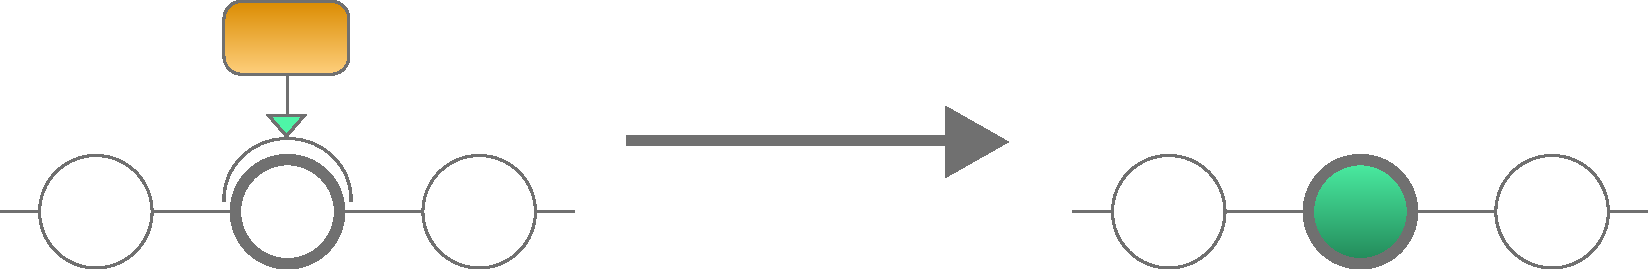
\includegraphics[width=\textwidth]{enzymes/random_a.pdf}
                        \end{minipage}
                        \vfill
                        \begin{minipage}{0.15\textwidth}
                            \caption*{\small \textbf{(b)}}
                        \end{minipage}
                        \begin{minipage}{0.8\textwidth}
                            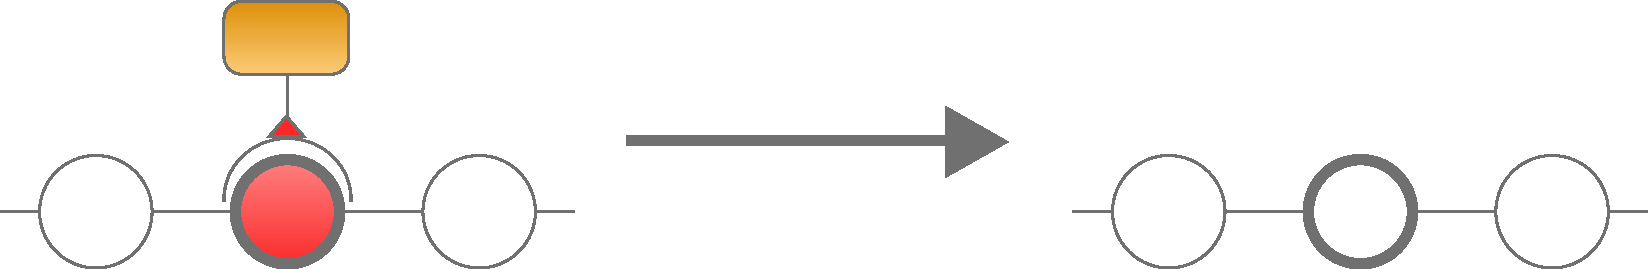
\includegraphics[width=\textwidth]{enzymes/random_b.pdf}
                        \end{minipage}
                    \end{minipage}
                    \caption{Simplified model of random modifier enzyme \textbf{(a)} acetylation addition \textbf{(b)} and methylation removal reactions. Acetylated nucleosomes are coloured in green, methylated nucleosomes are red and colourless ones are unmodified. Random modifier enzyme methylation addition and acetylation removal work analogically.}
                    \label{img:randomEnzymes}
                \end{figure}
                %

                %
                Random modifier enzymes' patterns do not have a context. However, a random methylation adder cannot bind to any already modified nucleosome, only to an unmodified one.
                %

                %
                Random modifier enzymes are not only “enzymes” in the true sense of the word when compared to the biological aspect of the model. They also exist in order to mimic the “noise” that is associated with such systems. Given that any nucleosome can be targeted by a specific random enzyme at any moment, these enzymes' association rate should be smaller than the other ones' in the system when trying to keep noise levels low.
                %
            %
            %
        %
        %
        \subsection{Enzyme rule sets}
            %
            This subsection provides an overview of the different enzyme rule sets used in the different simulations featured in this work. The rule sets are always kept constant throughout every section in the 'Results' chapter respectively, unless stated otherwise. The enzyme rule sets used are summarized in tab. \ref{tab:EnzymeRuleSets}.
            %

            %
            \begin{table}[htbp!]
                \centering
                \caption{Summary on whether an enzyme type was included and if the chromatin string was cyclic or not in the designated experiment presented in the indicated 'Results' section. \textbf{X} designates an affirmation.}
                \begin{tabular}{l|ccccc}
                                            & \ref{sec:ResNon-cooperative}  & \ref{sec:ResNonCyc} & \ref{sec:ResBistableSwitching}  & \ref{sec:ResBoundariesBistability}    \\\hline
                Random adders               & \textbf{X}                    & \textbf{X}          & \textbf{X}                      & \textbf{X}                            \\\hline
                Random removers             & \textbf{X}                    & \textbf{X}          & \textbf{X}                      & \textbf{X}                            \\\hline
                Linear adders               & \textbf{X}                    &                     &                                 &                                       \\\hline
                Linear removers             & \textbf{X}                    &                     &                                 &                                       \\\hline
                Cooperative adders          &                               & \textbf{X}          & \textbf{X}                      & \textbf{X}                            \\\hline
                Cooperative removers        &                               & \textbf{X}          &                                 &                                       \\\hline
                Cyclic                      &                               &                     & \textbf{X}                      & \textbf{X}                            \\\hline
                Non-cyclic                  & \textbf{X}                    & \textbf{X}          &                                 &                                       \\\hline
                \end{tabular}
                \label{tab:EnzymeRuleSets}
            \end{table}
           %
    %
    %
    \section{Simulation details}
    \label{sec:simulationDetails}
        %
        The input files for the performed \ed/ simulations can be found at \cite{Krecké2021}. In general, every \ed/ run needs three files: a \textit{statefile}, a \textit{rulefile} and a \textit{paramfile}. The \textit{statefile} contains the starting state of the nucleosome string. The \textit{rulefile} contains all specifications to the enzymes: their patterns, the modification pattern, the association rate and the dissociation rate. The \textit{paramfile} holds general information about the simulation itself with the most important one being the simulation time. This numeric parameter sets the exit condition for the algorithm.
        %

        %
        The simulation time changes significantly between some runs. This is due to Gillespie's algorithm's event-based time approach. Changing the enzyme set can result in a significantly different number of possible reactions during the simulation which can lead to very short simulation step numbers. Thus, in order to grant statistically significant runs, the simulation time was increased for certain runs, if the overall run time was empirically found to be too short.
        %

        %
        Furthermore, for reasons of performance and storage space, the graphs included in the results section were made from simulations with different simulation time. Preprocessing for the heatmaps was significantly more expensive than the other plots. Therefore, heatmaps were generated from \textit{short} runs, whereas the other plots were generated from \textit{long} runs. Meaning:
        %

        %
        \begin{itemize}
            \item \textit{short}: Every step (event) is plotted and metadata are used to plot association numbers and relative binding time (resulting in heatmaps).
            \item \textit{long}: Only every 1000th step is plotted. Given that the system is chaotic thanks to the random nature of the algorithm, regular plotting (e.g. every 1000th data point) results in a smoothing of the histogram because the chosen data points are more representative for the underlying distribution. Thus, there is no need for varying the skip length of 1000 throughout a run.
        \end{itemize}
        %
    %
    %
%
%
\chapter{Results}
    \label{cha:results}
    %

    %
    \section{Bistability without cooperative enzymes}
        \label{sec:ResNon-cooperative}
        %

        %
        In this section, we consider systems which do not contain directly cooperative enzymes. Thus, all the enzymes in the system's rule set read at most one “read-only” nucleosome with a maximum space of zero from the nucleosome that is modified. The enzymes act on a non-cyclic nucleosome string.
        %

        %
        \subsection{Influence of noise}
            %
            As pointed out before, systems without cooperative enzymes can indeed be bistable. However, they are very sensitive to increased noise. This is illustrated in fig. \ref{img:nonCoopSim}. The enzymes featured in this system with their respective association rates are summarized in tab. \ref{img:enzymeRatesNoise}.
            %

            %
            \begin{table}[htbp!]
                \caption{Enzyme types that are included in the rule set for the run illustrated in fig. \ref{img:nonCoopSim} with their respective association rates. All enzymes' dissociation rates are at an equal rate of 100,000. The enzyme rule set is symmetrical, which means that every enzyme type exists in favour of acetylation as well as methylation at equal rates respectively.}
                \begin{center}
                    \begin{tabular}{l r}
                        \hline
                        \textbf{enzyme type} & \textbf{association rate} \\
                        \hline
                        random adder & 1, 100 or 10,000 (see fig. \ref{img:nonCoopSim})\\
                        random remover & 2 \\
                        linear adder & 40,000 (20,000 to either direction)\\
                        linear remover & 40,000 (20,000 to either direction)\\
                        \hline
                    \end{tabular}
                \end{center}
                \label{img:enzymeRatesNoise}
            \end{table}
            %

            %
            On a sidenote, it should be mentioned that, in order to guarantee reproducibility and truthfulness of the statements derived from this kind of plots, it was always tried to ensure that the state distribution indicated by the histograms in the figures were as similar to each other as possible. Therefore, the simulations were always repeated numerous times with identical parameters (same rule set, same starting string, etc.). When the histograms were not similar in-between simulations, the simulation time was increased until similar histograms were achieved with every simulation.
            %

            %
            \begin{figure}[htpb!]
                \centering
                \begin{minipage}{\textwidth}
                    \begin{minipage}{0.1\textwidth}
                        \caption*{\small \textbf{(a)}}
                        % \label{}
                    \end{minipage}
                    \begin{minipage}{0.85\textwidth}
                        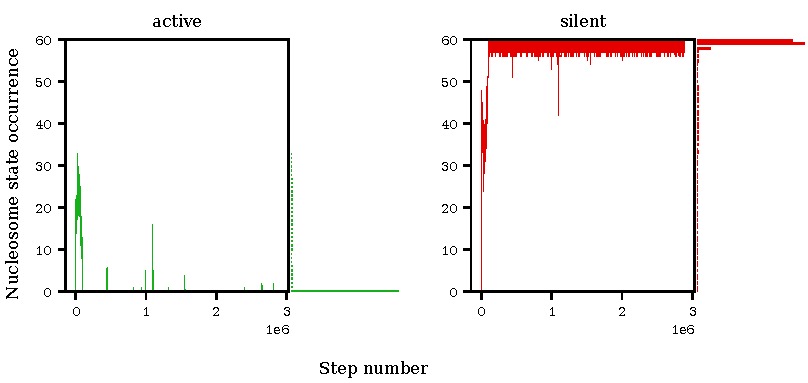
\includegraphics[width=\textwidth]{Results/4.1.1/peculiarCase4_0_runHistoryPlot_edited.pdf}
                        % \label{}
                    \end{minipage}
                \end{minipage}
                \begin{minipage}{\textwidth}
                    \begin{minipage}{0.1\textwidth}
                        \caption*{\small \textbf{(b)}}
                    \end{minipage}
                    \begin{minipage}{0.85\textwidth}
                        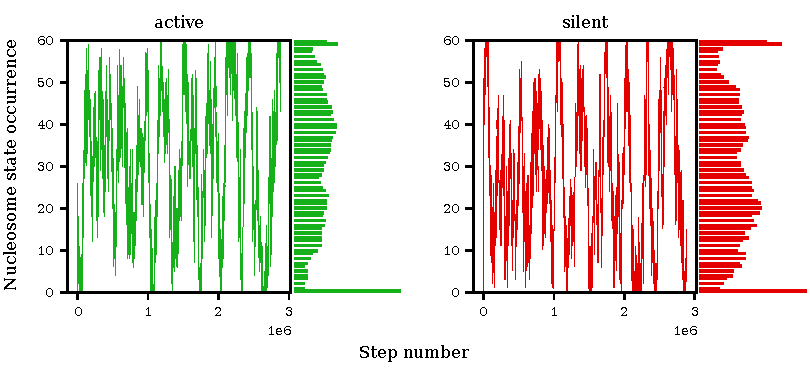
\includegraphics[width=\textwidth]{Results/4.1.1/peculiarCase2_edited.pdf}
                    \end{minipage}
                \end{minipage}
                \begin{minipage}{\textwidth}
                    \begin{minipage}{0.1\textwidth}
                        \caption*{\small \textbf{(c)}}
                        % \label{}
                    \end{minipage}
                    \begin{minipage}{0.85\textwidth}
                        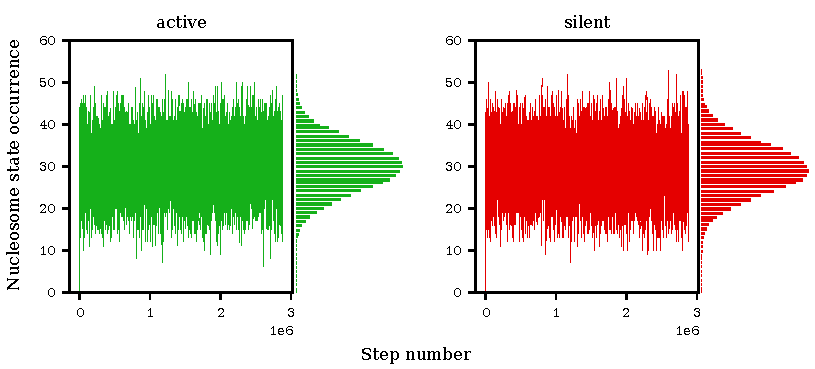
\includegraphics[width=\textwidth]{Results/4.1.1/peculiarCase3_1_runHistoryPlot_edited.pdf}
                        % \label{}
                    \end{minipage}
                \end{minipage}
                \caption{Absolute number of nucleosome states (active in green, silent in red) during the course of one long simulation (about 3 million reaction steps). Only every 1000th step is depicted. The enzyme rule set contains linear adders, random adders and random removers. The rule set does not contain cooperative enzymes. The enzymes' association rates are — linear adders: 40000 (20000 to each side), random removers: 2 and random adders: \textbf{(a)} 1, \textbf{(b)} 100, \textbf{(c)} 10000}
                \label{img:nonCoopSim}
            \end{figure}
            %

            %
            \begin{figure}[t!]
                \centering
                \includerunplot{Results/4.1.1/higherRandRemoverRates.pdf}
                \caption{Absolute number of nucleosome states (active in green, silent in red) during the course of one long simulation (about 4 million reaction steps). The enzyme rule set contains linear adders, linear removers, random adders and random removers. The rule set does not contain cooperative enzymes.}
                \label{img:nonCoopSim_bonus}
            \end{figure}
            %

            %
            In case \textbf{(a)} of fig. \ref{img:nonCoopSim}, at very low noise levels, one can easily see that the predominant state (here the silencing one) is stabilized. That said, no bistability is observed per se. However, it was found in additional simulation runs that the active state could just as easily turn out as the predominant state for the entire run. This fact seems rather logical as the starting state is a completely unmodified string and the used enzyme rule set is purely symmetrical, which means that it does not lean towards any of the two states concerning the association and dissociation rates.
            %

            %
            In case \textbf{(b)}, after increasing noise levels, the lack of resistance against noise gets clearer. As there are clearly two sharply defined most prevalent states with the chromatin string either fully acetylated or fully methylated, it might be tempting to call the system bistable. However, in sum, the states in between these extreme states are populated much more often, which makes the bistability in this system quite weak and not really applicable as something resembling a switch in a biological system.
            %

            %
            Finally, in case \textbf{(c)} with the random adders' association rate as close as $\nicefrac{1}{4}$ of the linear adders' and therefore considerably high noise levels, no bistability whatsoever can be observed any more. The histogram which counts the occurrence of active and silent nucleosomes respectively within the string shows a unimodal distribution throughout the simulation which is a “random walk”-like pattern on a fully modified string. The string is fully-modified because the dissociation rates are high compared to the association rates. The random modifications originate from overwhelming activity of the random enzymes. Accordingly, the nucleosome string states achieved during the simulation indeed disclose a monostable system.
            %

            %
            Increasing the random removers' rates results in more noise as well. This can be seen in fig. \ref{img:nonCoopSim_bonus} where the same enzyme rule set as in case \textbf{(b)} of fig. \ref{img:nonCoopSim} was used, except that the random removers' rates were raised from 2 to 100. In this case, the random walk area seems to have grown bigger and the string's full methylation or acetylation have both become extremely unstable.
            %
        %
        %
        \subsection{Bistability through indirect cooperativity}
            \label{subsec:indirectCoop}
            %

            %
            In a system of exclusively non-cooperative enzymes  with association rates indicated in table \ref{img:enzymeRatesPeculiarCase}, quite frequent bistability can indeed occur by adding linear removers to the rule set that was used in the example above.
            %

            %
            \begin{table}[htbp!]
                \caption{Enzyme types that are included in the rule set for the run illustrated in fig. \ref{img:outlook_nonCoop} with their respective association rates. All enzymes' dissociation rates are at an equal rate of 100,000. The enzyme rule set is symmetrical, which means that every enzyme type exists in favour of acetylation as well as methylation at equal rates respectively.}
                \begin{center}
                    \begin{tabular}{l r}
                        \hline
                        \textbf{enzyme type} & \textbf{association rate} \\
                        \hline
                        random adder & 100 \\
                        random remover & 2 \\
                        linear adder & 40,000 (20,000 to either direction)\\
                        linear remover & 40,000 (20,000 to either direction)\\
                        \hline
                    \end{tabular}
                \end{center}
                \label{img:enzymeRatesPeculiarCase}
            \end{table}
            %

            %
            \begin{figure}[htpb!]
                \centering
                \includerunplot{Results/4.1.2/StrongExtenders_cyclic_1_runHistoryPlot.pdf}
                \caption{Absolute number of nucleosome states (active in green, silent in red) during the course of one long simulation (about 1 million reaction steps). The enzyme rule set contains linear adders, linear removers, random adders and random removers. The rule set does not contain cooperative enzymes.}
                \label{img:outlook_nonCoop}
            \end{figure}
            %

            %
            The state adoption in this system resembles bistable behaviour as can be seen in fig. \ref{img:outlook_nonCoop}. One can clearly see that there are two very distinct peaks at complete activation and complete silencing of the nucleosome string.
            %

            %
            This bistability is most probably due to the fact that this system can now achieve indirect cooperativity. In a first step one, the linear remover reads two next-neighbour nucleosomes of opposite modification and, upon dissociation, leaves one of these unmodified. In step two, a linear adder modifies this nucleosome (through the usual read and write process) after reading a modified nucleosome next to it. This two-step process involves three nucleosomes in total which fulfills the condition for indirect cooperativity. It remains debatable if it is important, if the “read-only” nucleosomes are really different ones or if they may even be one and the same, resulting in the total involvement of merely two nucleosomes.\\
            %

            %
            Even though this system is bistable, however, it shows lack of variance around the peaks in the histogram.
            %

            %
            The histogram's peak variance can be understood as the area where the system has a more or less strong tendency to return to the peak's state.
            %

            %
            This behaviour is not observed in the indirectly cooperative case described in fig. \ref{img:outlook_nonCoop}. Thus, one single opposite modification added randomly to the string might entail the system's return to a random walk. As the term “stability” describes a state's resistance against small deviations and the addition of one single modification is nothing more than an atomic deviation for this system, one can say that this indirectly cooperative case does not qualify as a really robustly bistable system.
            %

            %
            Nonetheless, it is an interesting phenomenon overall, as it remains a theoretically useful switch-like concept that might find use in the biological context.
            %
            %
        %
        %
    %
    %
    \clearpage
    \section{Direct cooperativity and bistability on a non-cyclic string}
        \label{sec:ResNonCyc}
        %
        \subsection{Impact of cooperative enzymes}
            \label{subsec:impactOfCooperativeEnzymes}
            %
            Contrarily to section \ref{sec:ResNon-cooperative}, the simulations described in this section do contain cooperative adders and removers in the enzyme sets. In order to keep the rule sets as simple as possible, linear adders and removers are excluded from the enzyme set. Accordingly, other than cooperative enzymes, the rule set only contains random adders and removers.
            %

            %
            \begin{figure}[htpb!]
                \centering
                \includerunplot{Results/3.2_nonCyclString/shortRun_nonCyclic_highDiss_wCoopRem_4_runHistoryPlot.pdf}
                \caption{Absolute number of nucleosome states (active in green, silent in red) during the course of one simulation (about 56000 reaction steps). The enzyme rule set contains cooperative adders, cooperative removers, random adders and random removers. The amount of reaction steps is significantly lower than in fig. \ref{img:nonCoopSim} in order to be able to plot the heatmaps in figs. \ref{img:nonCyclBistability_bindingNumbers} and \ref{img:nonCyclBistability_bindingTimeDuration} with the data set from the same simulation.}
                \label{img:nonCyclBistability_runPlot}
            \end{figure}
            %

            %
            \begin{figure}[htpb!]
                \centering
                \includeheatmap{Results/3.2_nonCyclString/shortRun_nonCyclic_highDiss_wCoopRem_4_bindingNumbers}
                \caption{Heatmap depicting the absolute numbers of enzyme associations per enzyme and per nucleosome on the nucleosome string. The numbers originate from the same simulation plotted in fig. \ref{img:nonCyclBistability_runPlot}.}
                \label{img:nonCyclBistability_bindingNumbers}
            \end{figure}
            %

            %
            \begin{figure}[htpb!]
                \centering
                \includeheatmap{Results/3.2_nonCyclString/shortRun_nonCyclic_highDiss_wCoopRem_4_bindingTimeDuration}
                \caption{Heatmap depicting the average enzyme binding duration per enzyme and per nucleosome on the nucleosome string. The duration is defined as the number of time steps the enzyme has bound to one and the same nucleosome without dissociation event taking place in between divided by the total simulation time. The numbers originate from the same simulation plotted in fig. \ref{img:nonCyclBistability_runPlot}.}
                \label{img:nonCyclBistability_bindingTimeDuration}
            \end{figure}
            %

            %
            Figs. \ref{img:nonCyclBistability_runPlot}, \ref{img:nonCyclBistability_bindingNumbers} and \ref{img:nonCyclBistability_bindingTimeDuration} are derived from one same simulation with an enzyme rule set that contains the two cooperative enzyme types.
            %

            %
            One can easily see in fig. \ref{img:nonCyclBistability_runPlot} that with the newly added enzymes the predominant state (here the silencing one) is stabilized. It was found in additional simulation runs (see appendix \ref{app:additionalRuns}) that the active state might just as easily be the predominant state for the entire run, comparable to the indirect cooperativity case explained in \ref{subsec:indirectCoop}.
            %

            %
            It is important to note, that the histogram in fig. \ref{img:nonCyclBistability_runPlot} shows some variance around the peaks which is an important condition for robust stability in the mathematical sense, contrarily to the findings in \ref{subsec:indirectCoop}. In other words, the nucleosome string resists small perturbations and is able to return to a state that mostly contains one type of modifications, which will from now on be called a \textit{complete} state.
            %

            %
            These facts, the system either \textit{stably} finding itself in a completely active as well as a completely silent state, show that robust bistability has been achieved with this enzyme set.\\
            %

            %
            Figs. \ref{img:nonCyclBistability_bindingNumbers} and \ref{img:nonCyclBistability_bindingTimeDuration} provide more insights into the underlying mechanisms of the system. They originate from the same data as fig. \ref{img:nonCyclBistability_runPlot} does. As for the notion of 'space' indicated for each cooperative enzyme, please refer to section \ref{subsubsec:coopEnzymes}. A few seemingly surprising factors are to be addressed here.
            %

            %
            Every cooperative enzyme type shows a trapeze-like shape originating from a decreasing writeable area on the string with increasing pattern reach. This observation is tied to the inability of the enzymes to look beyond the string borders. As the pattern size increases, the cooperative enzyme is more and more unable to write onto a nucleosome  increasingly further away from the border. This is an unwanted effect, as it remains doubtful if this reflects any behaviour that would be seen as such in a natural biological setting.\\
            %

            %
            Fig. \ref{img:nonCyclBistability_bindingTimeDuration} reveals that there is a big discrepancy between the binding time of some enzymes compared to others. As the dissociation rates of the enzymes are very high and, importantly, precisely equal for every enzyme, completely dark spots must mean, that no enzyme has been active on that specific nucleosome at all throughout this simulation. For instance, the cooperative acetylation adders only seem to have been active on some nucleosomes close to both borders. The rest of the variance must originate from the stochastic nature of the simulation. Thus, this kind of plot is very useful for determining, if an enzyme type has been active at all on a specific nucleosome.\\
            %

            %
            Referring to fig. \ref{img:nonCyclBistability_bindingNumbers}, it is clear to see that the absolute number of associations of the random methylation remover is quite constant on most of the nucleosomes. As \ed/ was used as simulation tool, it is made sure that there are no associations without a following reaction and dissociation. Thus, as the random modification remover's context is one single modified nucleosome, the association number of the random removers can be taken as a locator of the modification (i.e. methylation or acetylation) they are removing with quite acceptable efficiency. In other words, fig. \ref{img:nonCyclBistability_bindingNumbers}, which shows the amount of enzyme associations per enzyme and per nucleosome, directly indicates, where a modification type was most prevalent on the string.
            %

            %
            The methylation mark was predominant throughout the entirety of the simulation. Given that the mentioned adders and removers are most active the more acetylation marks are already on the string, it does not seem surprising that the cooperative acetylation adders and the cooperative methylation removers show relatively low activity. The interesting activity pattern of those two enzyme types suggests that the acetylation subpopulations that can be seen in fig. \ref{img:nonCyclBistability_runPlot} must have been prevalent at the borders of the string almost exclusively. This is supported by the fact that the random methylation remover shows reduced activity at the borders.
            %

            %
            Thus can be concluded that it is very unlikely for any acetylation area to occur in the middle of the string while methylation is predominant, because empty spaces originating from random methylation removers are immediately filled up by cooperative methylation adders. The borders of the string, however, have a blocking effect on the cooperative methylation adders because with increasing space value, the nearest nucleosome that can be modified by them moves further and further away from the string border. The very first and very last nucleosomes are not modifiable at all by cooperative enzymes, hence the generation of acetylation subpopulations on the string borders.
            %
            %
        %
        %
        \subsection{Bistable switching on a non-cyclic string}
            %
            Considering the biological implications of the system, it would be much more useful if the system could effectively switch from one state to another within the course of one simulation, i.e. without changing the enzyme types involved or their rates and without resetting the nucleosome string to a completely unmodified string.
            %

            %
            This \textit{bistable switching} phenomenon, although rare, can be observed with the rule set described above (see fig. \ref{img:nonCyclBistability_runPlot2}). With the rule set containing random adders, removers and cooperative adders and removers, the system shows a bimodal distribution originating from one single simulation. Bistable switching can be observed about once every 10th simulation. Among hundreds of simulations, very few showed more than one bistable switching.
            %

            %
            As can be seen in fig. \ref{img:nonCyclBistability_runPlot2} between the times 0.2 and 0.4, the system undergoes bistable switching rather slowly. It is quite hard to determine any points of no return on the upper or lower border of this saddle point.
            %

            %
            \begin{figure}[htpb!]
                \centering
                \includerunplot{Results/3.2_nonCyclString/shortRun_nonCyclic_highDiss_wCoopRem_2_runHistoryPlot.pdf}
                \caption{Absolute number of nucleosome states (active in green, silent in red) during the course of one simulation (about 56000 reaction steps). Every reaction step is depicted in the plot. The x-axis shows the reaction time given by Gillespie's algorithm. The enzyme rule set contains cooperative adders, cooperative removers, random adders and random removers. Bistable switching, as seen in the plot, is only observed in about every 10th simulation of comparable reaction step size. The amount of reaction steps is significantly lower than in fig. \ref{img:nonCoopSim} in order to be able to plot the heatmaps in figs. \ref{img:coopAssocBindingDuration} and \ref{img:coopAssocBindingNumbers} with the data set from the same simulation.}
                \label{img:nonCyclBistability_runPlot2}
            \end{figure}
            %

             %
             \begin{figure}[htpb!]
                \centering
                \includeheatmap{Results/3.2_nonCyclString/shortRun_nonCyclic_highDiss_wCoopRem_2_bindingTimeDuration}
                \caption{Heatmap depicting the average enzyme binding duration per enzyme and per nucleosome on the nucleosome string. The duration is defined as the number of time steps the enzyme has bound to one and the same nucleosome without dissociation event taking place in between divided by the total simulation time. The numbers originate from the same simulation plotted in fig. \ref{img:nonCyclBistability_runPlot2}.}
                \label{img:coopAssocBindingDuration}
            \end{figure}
            %

            %
            \begin{figure}[htpb!]
                \centering
                \includeheatmap{Results/3.2_nonCyclString/shortRun_nonCyclic_highDiss_wCoopRem_2_bindingNumbers}
                \caption{Heatmap depicting the absolute numbers of enzyme associations per enzyme and per nucleosome on the nucleosome string. The numbers originate from the same simulation plotted in fig. \ref{img:nonCyclBistability_runPlot2}.}
                \label{img:coopAssocBindingNumbers}
            \end{figure}
            %

            %
            In fig. \ref{img:coopAssocBindingDuration}, the main difference from fig. \ref{img:nonCyclBistability_bindingTimeDuration} in the previous subsection is that both cooperative adders have been active across the entirety of the string in the present simulation, which makes sense because both modifications were predominant at one point in time.
            %

            %
            As can be seen in fig. \ref{img:coopAssocBindingNumbers}, the random remover enzymes are by far the most active enzymes from the set in this simulation, followed by the random adder enzymes which mainly show activity at the string borders. Apart from the random enzymes, the cooperative acetylation adders were active across the whole string while the other cooperative enzymes only were most active at the borders. Another interesting detail is that the cooperative methylation adders' activity looks a little stronger from nucleosome 30 onward to 60 than on the other half of the string. This behaviour could be recreated several times in other simulations where bistable switching occurred.
            %

            %
            As already pointed out in \ref{subsec:impactOfCooperativeEnzymes}, the acetylation mark must have taken over starting from the string borders, hence the intense enzymatic activity at these areas. The asymmetrical activity level of the cooperative methylation adders is particularly indicative of how and from where exactly the acetylation mark must have taken over. As the system reaches the saddle point, the acetylation area must probably have progressed all the way to the centre of the string from the left (i.e. nucleosome 1) rendering the cooperative methylation adder particularly inactive in this area for \nicefrac{1}{5} of the simulation time. It is likely that the opposite effect was not seen on the cooperative acetylation adders' activity pattern because the acetylation modification is prevalent for a longer time span (about \nicefrac{3}{5}), whereas the predominance period of the methylation modification is about as long as the system's prevalence periods in  proximity to the saddle point (about \nicefrac{1}{5}). These fraction indications are consistent even when looking at the absolute reaction step numbers. They are not distorted by the event-based time incrementation of Gillespie's algorithm.
            %
        %
        %
        \subsection{Bivalent switching on a non-cyclic string}
            %

            %
            In other simulations with the same settings as above (i.e. same enzyme rule set, starting state and simulation parameters), both modification levels meet close to the saddle point around 30 nucleosomes for quite a while before one modification turns out to be the predominant state again.
            %

            %
            \begin{figure}[htpb!]
                \centering
                \includerunplot{Results/3.2_nonCyclString/321_longRun_nonCyclic_highDiss_wCoopRem_01_runHistoryPlot.pdf}
                \caption{Absolute number of nucleosome states (active in green, silent in red) during the course of one simulation (about 175000 reaction steps). Every reaction step is depicted in the plot. The x-axis reaction step number. The enzyme rule set contains cooperative adders, cooperative removers, random adders and random removers.}
                \label{img:nonCyclBistability_runPlot3}
            \end{figure}
            %

            %
            The macrostate switching phenomenon shown in fig. \ref{img:nonCyclBistability_runPlot3} cannot be described as a "direct transition", which disqualifies it from being bistable switching (as it was defined in \ref{sec:TheoBistableSwitching}). Much rather, this phenomenon could be described as \textit{bivalent switching}, where the area around the saddle point is the pseudostable “STANDBY” state from which the system can evolve in either a completely active or silent macrostate. Clearly, the idea of \textit{irreversibility} (originating from the observation of bivalency in the context of generally unidirectional cell differentiation) is not reflected in this system.
            %

            %
            \begin{figure}[htpb!]
                \centering
                \includeheatmap{Results/3.2_nonCyclString/321_longRun_nonCyclic_highDiss_wCoopRem_01_bindingNumbers}
                \caption{Heatmap depicting the absolute numbers of enzyme associations per enzyme and per nucleosome on the nucleosome string. The numbers originate from the same simulation plotted in fig. \ref{img:nonCyclBistability_runPlot3}.}
                \label{img:coopAssocBindingNumbers_runPot3}
            \end{figure}
            %

            %
            In fig. \ref{img:coopAssocBindingNumbers_runPot3}, an asymmetrical activity pattern can be seen for the cooperative \ac/ adders as well as the random \ac/ removers. Both were quite a bit more active from nucleosome position 1 to 30 than on the other half of the chromatin string, while the random \me/ remover shows the exact opposite pattern. Again, given that the SSA does not allow dissociation without preoccuring reaction, it is certain to say that the left (1 - 30) half of the chromatin string contained \ac/ modifications more often throughout the simulation, while the right (31 - 60) half contained \me/ modifications more often.
            %

            %
            Like before, it is convenient to conclude that as soon as the saddle point was reached, there were two quite clearly separated areas present on the string: the \ac/ modification on one side and the \me/ modification on the other leaving both modifications at about equal possibility of taking over to be the predominant macrostate.
            %

            %
            Many of the phenomena discussed in this section originated from the linearity of the nucleosome string. As such, it presents two borders which, as was pointed out, have massive impacts on the enzymes' activity and also bistability. As these borders hardly seem justifiable from a biological point of view, it would be interesting and much more relevant biologically to achieve bistable switching on a nucleosome string without borders. This will be examined in the next section.
            %

            %
        %
        %
    %
    %
    \clearpage
    \section{Bistable switching on a cyclic string}
        \label{sec:ResBistableSwitching}
        %

        %
        \subsection{Achieving bistable switching}
            %
            %
            As was pointed out before, a linear nucleosome string with a finite number of nucleosomes that is reduced of length because of computational feasibility might not be best when aiming at designing a most general model that shows bistable switching. The drawbacks due to border effects of such a non-cyclic chain are evident as of the previous sections.
            %

            %
            \begin{figure}[htpb!]
                \centering
                \includerunplot{Results/3.3_bistableSwitching/longRun_cyclic_highDiss_wCoopRem_1_runHistoryPlot.pdf}
                \caption{Absolute number of nucleosome states (active in green, silent in red) during the course of one long simulation (about 678 million reaction steps). Only every 1000th step is depicted. The enzyme rule set contains random adders, random removers, cooperative adders and cooperative removers.}
                \label{img:cyclWCoopRem_runPlot1}
            \end{figure}
            %

            %
            \ed/ provides a means to work with circular nucleosome chains by establishing a direct next-neighbour relationship between the very first and very last nucleosome in the string. This method was used from this point on in the rest of the work. As border effects could now be effectively excluded, the nucleosome string length was reduced from 60 to 40 in order to lower computation expenses. It was made sure that the enzymes' maximum reach in the system was always low enough in order for the reduced string length not to trigger interlacing effects.
            %

            %
            With the borders eliminated, no bistable switching could be observed any more (see fig. \ref{img:cyclWCoopRem_runPlot1}). After one of the 2 modification types turns out predominant, it stays like this throughout the simulation with very little variance. This was to be expected, as the string borders helped the non-predominant modification to stay on the string end in the first place before growing its area across up to the other end of the string. As was pointed out in the previous section, the cooperative removers are much too strong for a non-prevalent modification to survive long enough without the protecting borders.\\
            %

            %
            The logical next step was to remove the cooperative removers from the rule set altogether. As can be seen in figs. \ref{img:cyclBistability_runPlot1} and \ref{img:cyclBistability_runPlot2}, this step was decisive for obtaining bistable switching on a cyclic string.
            %

            %
            \begin{figure}[htpb!]
                \centering
                \includerunplot{Results/3.3_bistableSwitching/longRun_cyclic_highDiss_noCoopRem_1_runHistoryPlot.pdf}
                \caption{Absolute number of nucleosome states (active in green, silent in red) during the course of one long simulation (about 634 million reaction steps). Only every 1000th step is depicted. The enzyme rule set contains random adders, random removers and cooperative adders (no cooperative removers).}
                \label{img:cyclBistability_runPlot1}
            \end{figure}
            %

            %
            \begin{figure}[htpb!]
                \centering
                \includerunplot{Results/3.3_bistableSwitching/longRun_cyclic_highDiss_noCoopRem_2_runHistoryPlot.pdf}
                \caption{Absolute number of nucleosome states (active in green, silent in red) during the course of one long simulation (about 634 million reaction steps). Only every 1000th step is depicted. The enzyme rule set contains random adders, random removers and cooperative adders (no cooperative removers).}
                \label{img:cyclBistability_runPlot2}
            \end{figure}
            %

            %
            As can be seen in these two figs., the removal of the cooperative removers not only entails the reappearance of bistable switching. Moreover, bistable switching is much more frequent in the simulations so much so that even multiple switchings in one simulation are not rare events any more. One can also see that the histogram peaks moved a bit closer towards the axis centre of 20 which means that the most stable states are not complete states any more. Instead, there is always a considerable subpopulation of about 10\% of the opposite modification present, showing high variance.
            %

            %
            Although the system passes the saddle point around 20 nucleosomes quite often, it seems that this state is never populated for a very long time, as is shown by figs. \ref{img:cyclBistability_runPlot1} and \ref{img:cyclBistability_runPlot2}. Accordingly, the point of no return seems much more narrow than in the linear case with cooperative removers present in the rule set.\\
            %
            %
        %
        %

        \subsection{Length of macrostates}
            \label{subsec:macrostateLength}
            %
            %
            As bistable switching has become a quite common phenomenon in this setting, it seems tempting to calculate the average \textit{macrostate length}, with the macrostate defined as the current predominant modification state. In order to do so, for each simulation out of 150 with total step numbers of about 650,000 respectively, every macrostate length was counted. The macrostate started when at least 75\% of the nucleosomes on the string presented one same modification, and it ended when the opposite modification was present on 75\% of the nucleosomes. This implies that the “transition” states around the saddle point are included in the macrostate lengths. However, this was considered to be acceptable given that the transitions in this system are quite negligeable concerning their relative duration and the resulting inclusion of transition states is equally distributed for \me/ as well as \ac/ macrostates.
            %

            %
            Also, all macrostates that lasted up until the end of the simulation were not counted because the duration of said macrostates could not be accurately determined as their end was not yet reached at the end point of the simulation. Accordingly, macrostates from simulations which did not show any bistable switching were discarded.
            %

            %
            \begin{figure}[htpb!]
                \begin{minipage}{.69\textwidth}
                    \centering
                    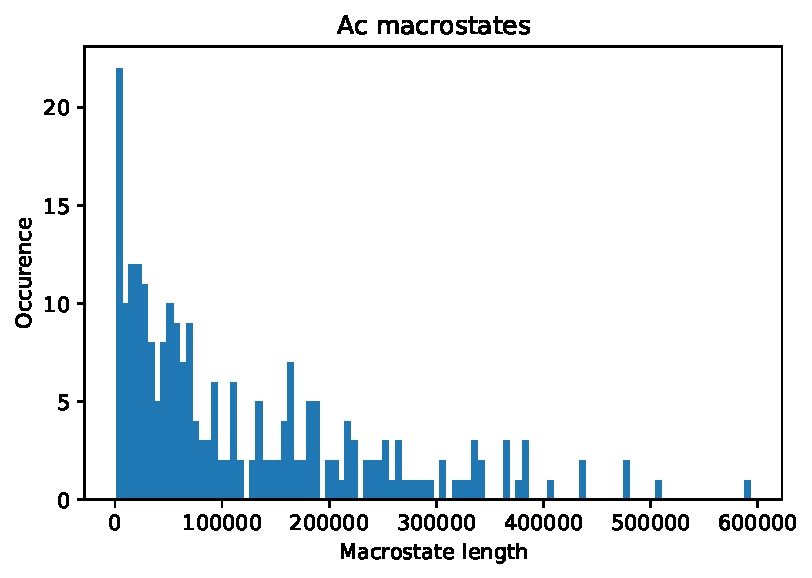
\includegraphics[width=\textwidth]{Results/3.3_bistableSwitching/macrostate_length_hist.pdf}
                    \caption*{\textbf{(a)}}
                \end{minipage}
                \begin{minipage}{.29\textwidth}
                    \centering
                    \begin{tabular}{rr}
                        count	& 243.000 \\
                        mean	& 119779.021 \\
                        % std	    & 118142.252 \\
                        min	    & 1180.000 \\
                        25\%	& 26212.500 \\
                        50\%	& 71719.000 \\
                        75\%	& 182782.000 \\
                        max	    & 593180.000 \\
                    \end{tabular}
                    \caption*{\textbf{(b)}}
                \end{minipage}
                \caption{\textbf{(a)} Histogram counting the acetylation macrostates' lengths of a system with identical settings as the one described at the beginning of this section. \textbf{(b)} Statistical data of the acetylated macrostates}
                \label{img:cyclBistability_hist}
            \end{figure}
            %

            %
            \noindent
            A data summary of the findings can be seen in fig. \ref{img:cyclBistability_hist}.
            %

            %
            With a total count of 243 bistable switchings throughout the 150 simulations, the data abundance is quite scarce on the considerable value range of about 1000 up to almost 600,000. Additionally, the mean value of about 119,779 seems quite far away from the most frequent value range, which makes an underlying Poisson distribution unlikely. Besides this, because of the high complexity of the collected data, it does not seem trivial to determine if the macrostate length is a Poisson process at all.
            %

            %
            Regardless, more data would be needed in order to be able to perform solid statistical analyses. However, achieving the needed amount of data seems unfeasible with the present computational and timely resources of the author.
            %
        %
        %
        \subsection{Enzyme contributions per macrostate}
            %
            %
            In order to get more insights into the macrostates' influence on the enzymes, the macrostate dependent activity of the random and cooperative adders was analysed by differentiating between three nucleosome string state categories: the \ac/ macrostate (>75\% of nucleosomes on the string are acetylated), the \me/ macrostate (>75\% of nucleosomes on the string are methylated) and the grey area closer around the saddle point which holds all other states. For convenience reasons, these three categories will be referred to as macrostates of the system which includes the grey area in this context.
            %

            %
            String states which show more than 25\% of unmodified nucleosomes were not taken into account. However, such cases were only discovered at the beginning of the simulation.
            %

            %
            For the macrostates separately, the adder enzyme counts were summarized over the same 150 simulations of around 600,000 simulation steps as above. The enzyme association rates are 140,000 for the cooperative adders (20,000 for every differently spaced rule), 10,000 for the random adders and 2 for the random removers. The percentage of enzymatic adder activity is summarized in tab. \ref{tab:cyclBistability_enzymes}.
            %

            %
            \begin{table}[htpb!]
                \centering
                \caption{Macrostate dependent adder enzyme binding event counts in percent. \textit{Me} refers to the \me/ macrostate, \textit{Ac} to the \ac/ macrostate and Grey refers to the state in-between the two macrostates, where both modifications are prevalent on less than 75\% of the nucleosomes.}
                \begin{tabular}{lrrrrr}
                                &   CoopM	    &   CoopA       &   RandM       &   RandA   &   $\Sigma$  \\\hline
                    Me	        &   21.00\%	    &   0.21\%	    &   1.86\%	    &   1.85\%   &   24.91\%    \\
                    Grey        &   10.44\%	    &   10.49\%	    &   3.17\%	    &   3.18\%   &   27.28\%    \\
                    Ac	        &   0.21\%	    &   21.00\%	    &   1.85\%	    &   1.86\%   &   24.92\%    \\
                \end{tabular}
                \label{tab:cyclBistability_enzymes}
            \end{table}
            %

            % % equal amount of significant numbers
            % \begin{table}[htpb!]
            %     \centering
            %     \caption{Macrostate dependent adder enzyme binding event counts in percent. \textit{Me} refers to the \me/ macrostate, \textit{Ac} to the \ac/ macrostate and Grey refers to the state in-between the two macrostates, where both modifications are prevalent on less than 75\% of the nucleosomes.}
            %     \begin{tabular}{lrrrrr}
            %         Macrostate  &   CoopM	    &   CoopA       &   RandM       &   RandA   &   $\Sigma$  \\\hline
            %         Me	        &   21.00	    &   0.2053	    &   1.856	    &   1.854   &   24.91    \\
            %         Grey        &   10.44	    &   10.49	    &   3.166	    &   3.184   &   27.28    \\
            %         Ac	        &   0.2066	    &   21.00	    &   1.853	    &   1.857   &   24.92    \\
            %     \end{tabular}
            %     \label{tab:cyclBistability_enzymes}
            % \end{table}
            %

            %
            It might seem surprising at first that for every state category (Me, Grey, Ac), the overall adder binding event percentage is only around 25\%. However, this makes perfect sense because every enzyme binding event is followed by a reaction/dissociation step which will make up for about another 25\% of the overall event count. The remaining 50\% are probably due to random remover binding and removing activity.
            %

            %
            Other than that, the enzymes show expected symmetrical activity levels: the random enzymes are equally active in the \me/ macrostate as in the \ac/ macrostate and the cooperative \me/ adder is equally active in the \me/ macrostate as the cooperative \ac/ adder is in the \ac/ macrostate and vice versa.
            %

            %
            \begin{table}[htpb!]
                \centering
                \caption{Macrostate dependent modification events in percent. \textit{Me} refers to the \me/ macrostate, \textit{Ac} to the \ac/ macrostate and Grey refers to the state in-between the two macrostates, where both modifications are prevalent on less than 75\% of the nucleosomes.}
                \begin{tabular}{lrr}
                                &   Methylation	    &   Acetylation \\\hline%\hline
                    Me	        &   91.36\%	        &   8.26\% \\%\hline
                    Grey        &   49.86\%	        &   50.14\% \\%\hline
                    Ac	        &   8.27\%	        &   91.73\% \\
                \end{tabular}
                \label{tab:cyclBistabilities_modificationProb}
            \end{table}
            %

            %
            Tab. \ref{tab:cyclBistabilities_modificationProb} summarizes the respective \ac/ and \me/ modification rates for each macrostate based on the data from tab. \ref{tab:cyclBistability_enzymes}. Understandably, methylation and acetylation events happen at equal rates in the grey area, as the system can establish either \me/ or \ac/ macrostates from the saddle point. The rate of about 8\% of acetylation events in the \me/ macrostate (and vice versa) are consistent with the previous graphical estimation, that the respective subpopulations are to find on about 10\% of nucleosomes.
            %

            %
            \begin{table}[htpb!]
                \centering
                \caption{Macrostate dependent contributions of cooperative and random adders respectively in percent. \textit{Me} refers to the \me/ macrostate, \textit{Ac} to the \ac/ macrostate and Grey refers to the state in-between the two macrostates, where both modifications are prevalent on less than 75\% of the nucleosomes.}
                \begin{tabular}{l|rr|rr}
                                &   \multicolumn{2}{|c|}{Methylation}    & \multicolumn{2}{c}{Acetylation} \\
                                &   random	    &   cooperative     &   random      &   cooperative     \\\hline%\hline
                    Me	        &   8.12\%	    &   91.88\%         &   90.00\%     &   9.96\%  \\%\hline
                    Grey        &   23.28\%	    &   76.72\%         &   23.28\%     &   76.72\% \\%\hline
                    Ac	        &   89.95\%	    &   10.05\%         &   8.12\%      &   91.88\% \\
                \end{tabular}
                \label{tab:cyclBistabilities_enzymeProb}
            \end{table}
            %

            %
            Tab. \ref{tab:cyclBistabilities_enzymeProb} further breaks down the numbers in order to show the contributions of the different enzyme types, random and cooperative, for the respective macrostate. It is easier to see here that the numbers for methylation are equal to the inverted acetylation numbers.
            %

            %
            It was to expect that in all the macrostates, the effective association ratio between the cooperative adder and the random adder activity is different from the set one, because the cooperative enzymes' pattern includes more restrictions. Theoretically, given that the cooperative adders have a set association rate of 140,000 and the random adders' association rate is set at 10,000, one could expect that the random enzymes bind at least $\nicefrac{1}{14}$ as often as the cooperative adders. This is indeed observed for all three macrostates.
            %

            %
            Interestingly, the cooperative enzymes are about three times as active as the random adders in the grey area and still show an activity of $\nicefrac{1}{10}$ in the respective non-favoured macrostate. One would expect that, in an \ac/ dominated macrostate for instance, a cooperative \me/ adder might be able to read its pattern far less often given that the \me/ modification is only present in a relatively small subpopulation. A possible explanation is that the modifications are scattered very randomly along the chromatin string, in contrast to the non-cyclic case.
            %
            %
        %
        %
    %
    %
    \newpage
    \section{The boundaries of bistability}
        \label{sec:ResBoundariesBistability}
        %

        %
        \subsection{Influence of the dissociation rate}
            \label{subsec:ResInfluenceDissociationRate}
            %

            %
            In the previous sections, the system's parameter that was most focussed on were the enzyme types in the rule set. The dissociation rate, however, was kept at a very high rate. This section serves the purpose of examining, what happens if the dissociation events enter in concurrence with the associations throughout the simulation.
            %

            %
            \begin{figure}[htpb!]
                \centering
                \includerunplot{Results/3.4_dissocRate/longRun_cyclic_lowDiss_noCoopRem_3_runHistoryPlot_wSum.pdf}
                \caption{Absolute number of nucleosome states (active in green, silent in red, sum of active and silent in blue) during the course of one long simulation (about 126 million reaction steps). Only every 1000th step is depicted. The enzyme rule set contains random adders, random removers and cooperative adders (no cooperative removers).}
                \label{img:dissoc_runPlot1}
            \end{figure}
            %

            %
            \begin{figure}[htpb!]
                \centering
                \includerunplot{Results/3.4_dissocRate/longRun_cyclic_highDiss_noCoopRem_3_runHistoryPlot_wSum.pdf}
                \caption{Absolute number of nucleosome states (active in green, silent in red, sum of active and silent in blue) during the course of one long simulation (about 639 million reaction steps). Only every 1000th step is depicted. The enzyme rule set contains random adders, random removers and cooperative adders (no cooperative removers).}
                \label{img:dissoc_runPlot2}
            \end{figure}
            %

            %
            In the previous simulations, enzymes were bound for an average of two or three events before writing and dissociating from the bound nucleosome. Decreasing the dissociation rate inherently means a longer binding time on the nucleosome. Fig. \ref{img:dissoc_runPlot1} shows that this longer binding time entailed by a lower dissociation rate (100) has severe effects on the whole simulation outcome compared to a simulation with exactly the same parameters except for a 1000 times higher dissociation rate (100,000) for every enzyme (see fig. \ref{img:dissoc_runPlot2}).
            %

            %
            Fig. \ref{img:dissoc_runPlot1} discloses a much lower number of total reaction events during the simulation from fig. \ref{img:dissoc_runPlot1} compared to fig. \ref{img:dissoc_runPlot2}. Additionally, the most striking difference is that the adopted states histogram shows a monomodal distribution even though it is easy to see from fig. \ref{img:dissoc_runPlot2} that a bimodal distribution and, thus, bistability can be achieved with this enzyme set.
            %

            %
            It is evident that bistability, although possible from a rule set point of view, can be eliminated by a low dissociation rate. This is probably because during binding time, the enzymes are blocking the ability for other enzymes to bind to the same nucleosome and, in a way, act as protective groups. As a result, the number of possible events for each respective time step is massively reduced. This is also shown by the reduced overall event number in fig. \ref{img:dissoc_runPlot1}, as the SSA increases the time elapsed between events the lower the number of possible events is (see \ref{subsec:Gillespie}).
            %

            %
            An additional striking detail from fig. \ref{img:dissoc_runPlot1} is that the total number of modified nucleosomes is generally quite low compared to fig. \ref{img:dissoc_runPlot2}. It averages around 25 out of 40 nucleosomes which means that at any time during the simulation, around 15 nucleosomes on the string are unmodified. This probably happens because many association events are followed by reaction and dissociation rather lately.
            %

            %
            The protective behaviour of enzymes with low dissociation rate and the high number of unmodified nucleosomes are likely to be the main reasons for bistability not occuring in simulations with enzymes that have low dissociation rates. Cooperative adders are meant to take the dominating modification into account to act as the main drivers for bistability. With low dissociation rates, the presence of quite many unmodified nucleosomes as well as a slowed down modification velocity because of protective enzymes inhibit the cooperative adders and, thus, prevent bistability.
            %

            %
            Thus, it seems that the dissociation rate is an important influential factor that has to be taken into account or “eliminated” by raising its value high enough when trying to achieve bistability.
            %
        %
        %
        \subsection{Cooperative enzyme reach}
            \label{subsec:cooperativeEnzymeReach}
            %
            Another interesting property is the cooperative enzymes' reach , i.e. the space between the reading areas and the writing position.
            %

            %
            \begin{figure}[htpb!]
                \centering
                \begin{minipage}{0.77\textwidth}
                    \begin{minipage}{0.1\textwidth}
                        \caption*{\small \textbf{(a)}}
                        % \label{}
                    \end{minipage}
                    \begin{minipage}{0.65\textwidth}
                        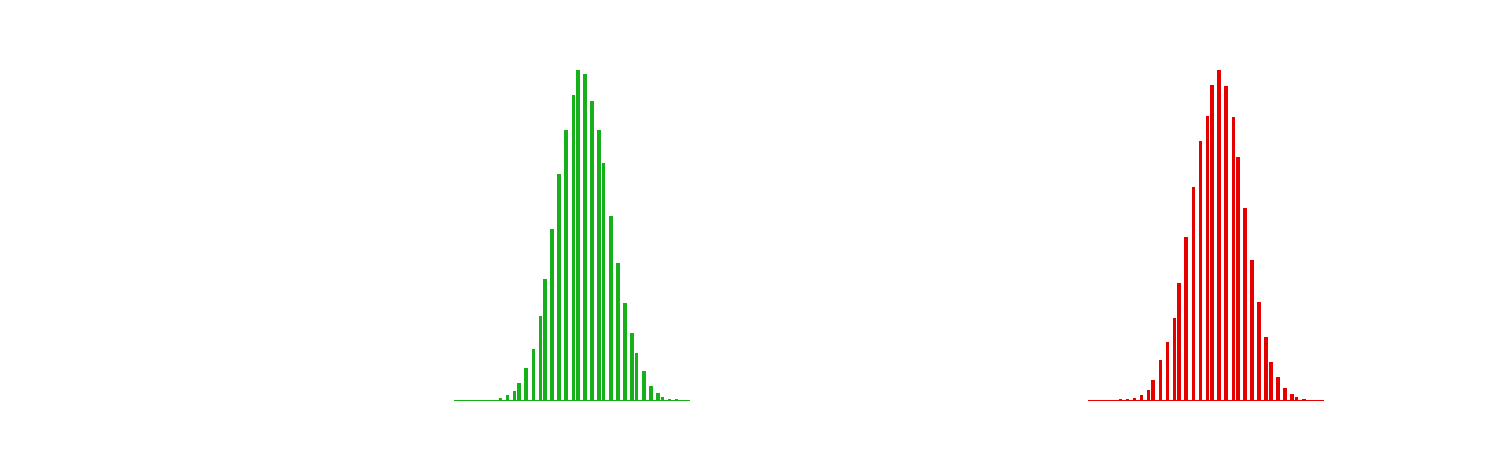
\includegraphics[width=\textwidth]{Results/3.5_boundariesBistability/maxReach0_0_HistogramPlot.pdf}
                        % \label{}
                    \end{minipage}
                \end{minipage}
                \begin{minipage}{0.77\textwidth}
                    \begin{minipage}{0.1\textwidth}
                        \caption*{\small \textbf{(b)}}
                    \end{minipage}
                    \begin{minipage}{0.65\textwidth}
                        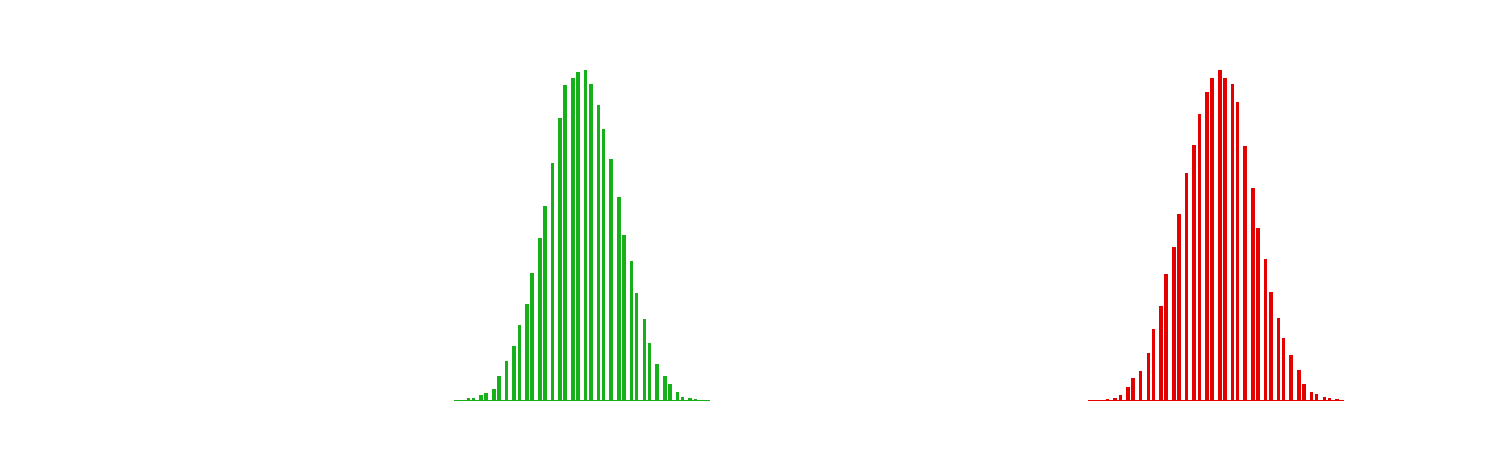
\includegraphics[width=\textwidth]{Results/3.5_boundariesBistability/maxReach1_4_HistogramPlot.pdf}
                    \end{minipage}
                \end{minipage}
                \begin{minipage}{0.77\textwidth}
                    \begin{minipage}{0.1\textwidth}
                        \caption*{\small \textbf{(c)}}
                        % \label{}
                    \end{minipage}
                    \begin{minipage}{0.65\textwidth}
                        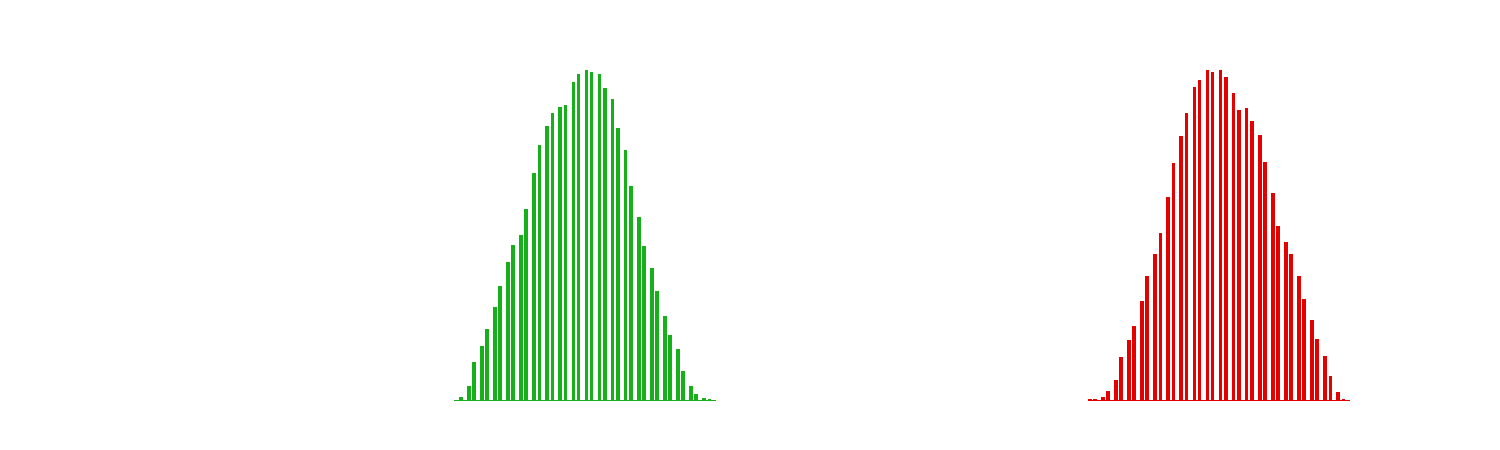
\includegraphics[width=\textwidth]{Results/3.5_boundariesBistability/maxReach2_2_HistogramPlot.pdf}
                        % \label{}
                    \end{minipage}
                \end{minipage}
                \begin{minipage}{0.77\textwidth}
                    \begin{minipage}{0.1\textwidth}
                        \caption*{\small \textbf{(d)}}
                    \end{minipage}
                    \begin{minipage}{0.65\textwidth}
                        
\includegraphics[width=\textwidth]{Results/3.5_boundariesBistability/maxReach3_3_HistogramPlot.pdf}
                    \end{minipage}
                \end{minipage}
                \begin{minipage}{0.77\textwidth}
                    \begin{minipage}{0.1\textwidth}
                        \caption*{\small \textbf{(e)}}
                        % \label{}
                    \end{minipage}
                    \begin{minipage}{0.65\textwidth}
                        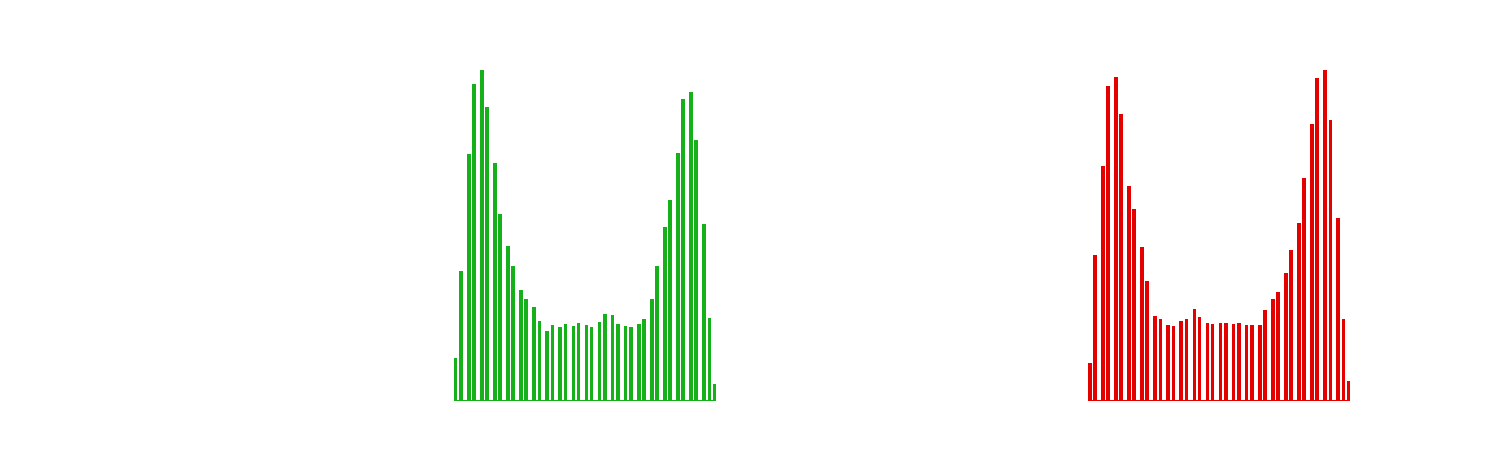
\includegraphics[width=\textwidth]{Results/3.5_boundariesBistability/maxReach4_3_HistogramPlot.pdf}
                        % \label{}
                    \end{minipage}
                \end{minipage}
                \begin{minipage}{0.77\textwidth}
                    \begin{minipage}{0.1\textwidth}
                        \caption*{\small \textbf{(f)}}
                    \end{minipage}
                    \begin{minipage}{0.65\textwidth}
                        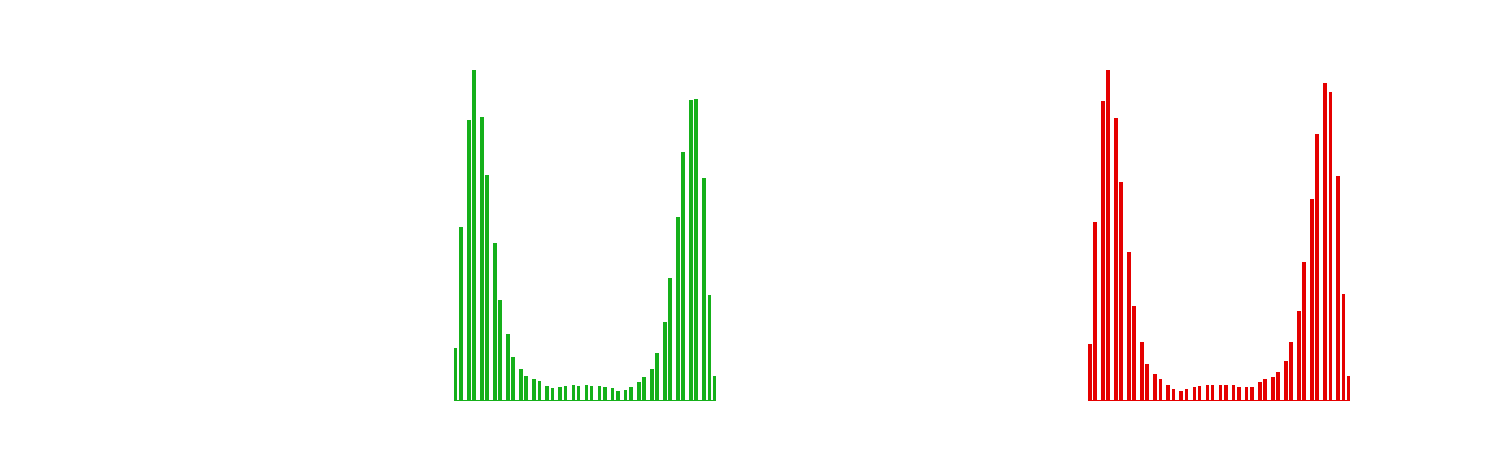
\includegraphics[width=\textwidth]{Results/3.5_boundariesBistability/maxReach5_4_HistogramPlot.pdf}
                    \end{minipage}
                \end{minipage}
                \begin{minipage}{0.77\textwidth}
                    \begin{minipage}{0.1\textwidth}
                        \caption*{\small \textbf{(g)}}
                    \end{minipage}
                    \begin{minipage}{0.65\textwidth}
                        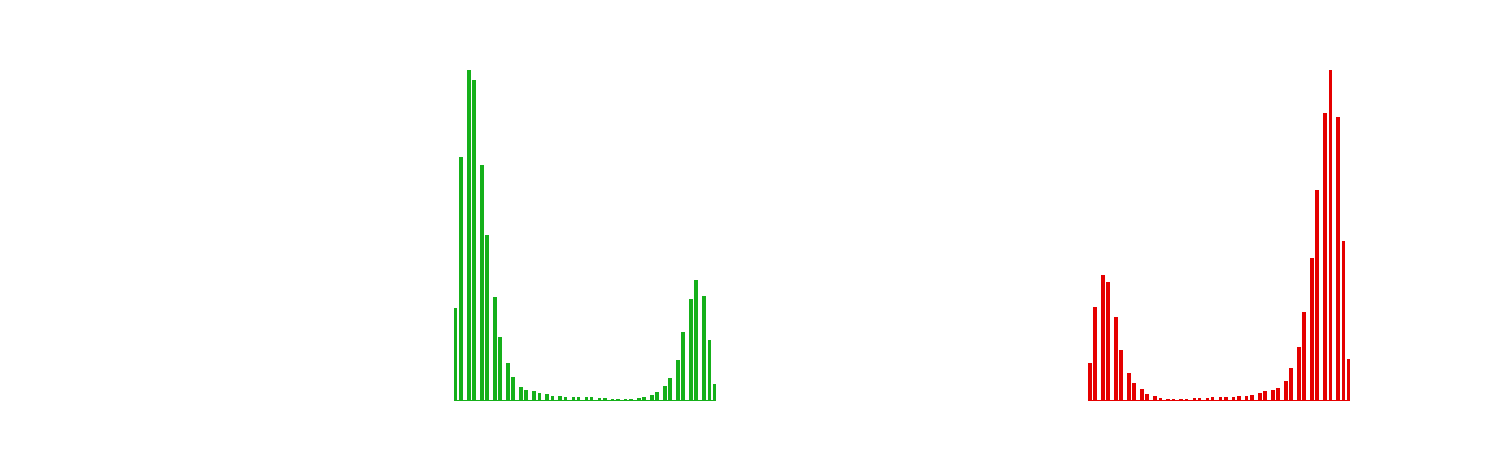
\includegraphics[width=\textwidth]{Results/3.5_boundariesBistability/maxReach6_4_HistogramPlot.pdf}
                    \end{minipage}
                \end{minipage}
                \caption{Histograms representing the absolute number of nucleosome states from 40 (left) to 0 (right) (active in green, silent in red, sum of active) during the course of one long simulation (about 638 million reaction steps). The enzyme rule set contains random adders, random removers and cooperative adders (no cooperative removers). The cooperative adders' maximum space is varied to be \textbf{(a)} 0, \textbf{(b)} 1, \textbf{(c)} 2, \textbf{(d)} 3, \textbf{(e)} 4, \textbf{(f)} 5 and \textbf{(g)} 6. Space is defined as the number of nucleosomes between the nucleosome which is read on either side and the unmodified nucleosome that is to be modified. The space to the left and right is always equal for every respective cooperative adder rule.}
                \label{img:enzymeReach}
            \end{figure}
            %

            %
            In all previous sections, cooperative adders constantly included rules with spaces of zero up to six. Space is defined as the number of nucleosomes between a “read-only” nucleosome and the nucleosome to be modified. The space is equal left and right of the nucleosome to be modified.
            %

            %
            Fig. \ref{img:enzymeReach} shows that the histograms of the absolute nucleosome state numbers change dramatically when varying the cooperative adders' space variable. Case \textbf{(a)} shows a monomodal distribution, which is to be expected because the cooperative adders in this system do not have a pattern that exceeds next-neighbour relations. As explained in \ref{subsec:multistable}, this fact makes bistability very hard up to impossible to achieve at considerable noise levels. It seems that for the present set of parameters, including the chromatin length of 40 nucleosomes, the present association rates of 140,000 (20,000 for each space rule) for cooperative adders, 10,000 for random adders and 2 for random removers and a universal dissociation rate of 100,000, a bimodal distribution is consistently achieved starting at a space of 4, as can be seen in case \textbf{(e)} of fig. \ref{img:enzymeReach}. In this case, the cooperative adders' biggest pattern contains 11 nucleosomes, including the nucleosome to be modified, having an overview across $\nicefrac{1}{4}$ of the entire nucleosome string.
            %

            %
            Naturally, no general statement can be given based on these findings as to how far cooperative adders with fixed “arm” lengths have to be able to “detect” modifications. However, it has become clear that fixed neighbour relations are not an unbreachable barrier when trying to achieve robust bistability or even bistable switching, provided the reach is far enough.
            %

            %
            Another interesting effect can be seen in cases \textbf{(e)}, \textbf{(f)} and \textbf{(g)}. For one, the saddle point seems less and less populated with increasing enzyme reach. Secondly, case \textbf{(g)} shows an asymmetrical distribution which might not be expected at first. Summarizing those two observations, it seems that the macrostates turn out to gain stability the higher the cooperative enzymes' reach is. As a result, one macrostate lasts longer than the other one in a simulation which results in an asymmetrical bimodal distribution. For example, in case \textbf{(g)} from fig. \ref{img:enzymeReach}, the active macrostate prevailed longer than the silent macrostate. Overall, the system is still symmetrical, as there are also simulations based on identical parameters which show the opposite picture with the silent macrostate being the longer lasting one.
            %

            %
            When choosing an even larger space value for the cooperative adders, the macrostates become more and more stable up to a point where bistable switching can only rarely be observed any more. As some simulations still show an acetylation macrostate whereas others show a methylation macrostate, the system is still bistable, regardless of the space value, provided the latter is above the value of four.
            %
            %
        %
        %
    %
    %
    % \newpage
    % \section{Bivalency}
    %     \label{sec:ResBivalency}
    %     %
    %     \begin{figure}[htpb!]
    %         \centering
    %         \includerunplot{Results/3.6_Bivalency/TotalComplete_example.png} % change this
    %         \caption{}
    %         % \label{img:dissoc_runPlot2}
    %     \end{figure}
    %     %
    %     \begin{figure}[htpb!]
    %         \centering
    %         \includerunplot{Results/3.6_Bivalency/BivalentComplete_example.png} % change this
    %         \caption{}
    %         % \label{img:dissoc_runPlot2}
    %     \end{figure}
    %     %
    %     \begin{figure}[htpb!]
    %         \centering
    %         \includerunplot{Results/3.6_Bivalency/BivalentBistability_example.png} % change this
    %         \caption{}
    %         % \label{img:dissoc_runPlot2}
    %     \end{figure}
    %     %
    %     \begin{itemize}
    %         {
    %             \color{red} %
    %             \item Here, we are at Kx+Ky
    %             \item Two systems that either favour bivalency or total active/silent states as an introduction to bivalency
    %             \item Frequent switching and bivalency
    %         }
    %     \end{itemize}
        %
    %
    %
%
%
\chapter{Discussion}
    \label{cha:discussion}
    %

    %
    This thesis showed in practical examples that establishing bistable nucleosome PTM systems with software like \ed/ which takes fixed nucleosomal neighbour relations into account is possible. As concluded by Dodd et al. \cite{dodd2007theoretical}, cooperative enzymes which non-locally “sense” the presence or absence of chemical modifications on the chromatin seem to be imperatively needed in order for the system to show robust bistability.\\
    %

    %
    In accordance with Dodd et al., the parameter space in which bistability through indirect cooperativity can be observed is indeed reduced compared to the directly cooperative counterpart. However, contrarily to Dodd et al.'s findings, indirect bistability, albeit non-robust, could be shown to exist in absence of high noise in the transition region, as shown in \ref{subsec:indirectCoop}.
    %

    %
    Furthermore, this work grants a proof of concept that bistability can be easily achieved with a partially non-local model which takes neighbour relations into account. As such, it offers the perspective of a hybrid model that unifies the rather traditional approach of strict next-neighbour relations and Dodd et al.'s approach of a fully fluid nucleosome string model. This might mark an important step towards a highly customizable model which can fulfill many requirements when trying to get closer to real-life biology.\\
    %

    %
    In this work, critical factors, which have substantial influence concerning the bistability of a system as well as the likelihood of bistable switching in a simulation were identified and qualitatively analyzed. A summary of the impact of every one of these parameters is provided below.\\
    %

    %
    % In the following discussion, a simplified landscape model is introduced in order to put the findings into perspective and provide a framework which simplifies further study of the various influential factors.
    %

    %
    Finally, based on the results from this work, the information known about the bistable switching mechanisms with cooperative enzymes is summarized for the non-cyclic as well as the cyclic case.
    %

    %
    %
    \section{Factors which influence bistability}
        %

        %
        % \subsection{A landscape model}
        %     %

        %     %
        %     In order to identify important influential factors concerning a dynamic histone PTM system, given the vast dimensionality of the parameter space, it seems convenient to provide a simplified model of such a system. Apart from serving as an illustrational tool, such a model is also quite helpful in pointing out the inadequacies one might overlook when trying to reduce such a system to its elementary components.
        %     %

        %     %
        %     In this simplified three-dimensional model, the x- and y-axes comprise the entirety of active and silent modification distributions on the nucleosome string. One such a distribution pattern is called a \textit{state}. The z-axis summarizes all influential factors that result in increased or decreased stability of a certain state in a specific point in time. These factors include all the association and dissociation rates, as well as the types of enzymes in the rule set. Stable states are those, that are adopted in the majority of time steps throughout the simulation.\\
        %     %

        %     %
        %     \begin{figure}[!htpb]
        %         \centering
        %         \begin{minipage}[t]{\textwidth}
        %             \begin{minipage}{0.19\textwidth}
        %                 \caption*{\small \textbf{(a)}}
        %             \end{minipage}
        %             \begin{minipage}{0.8\textwidth}
        %                 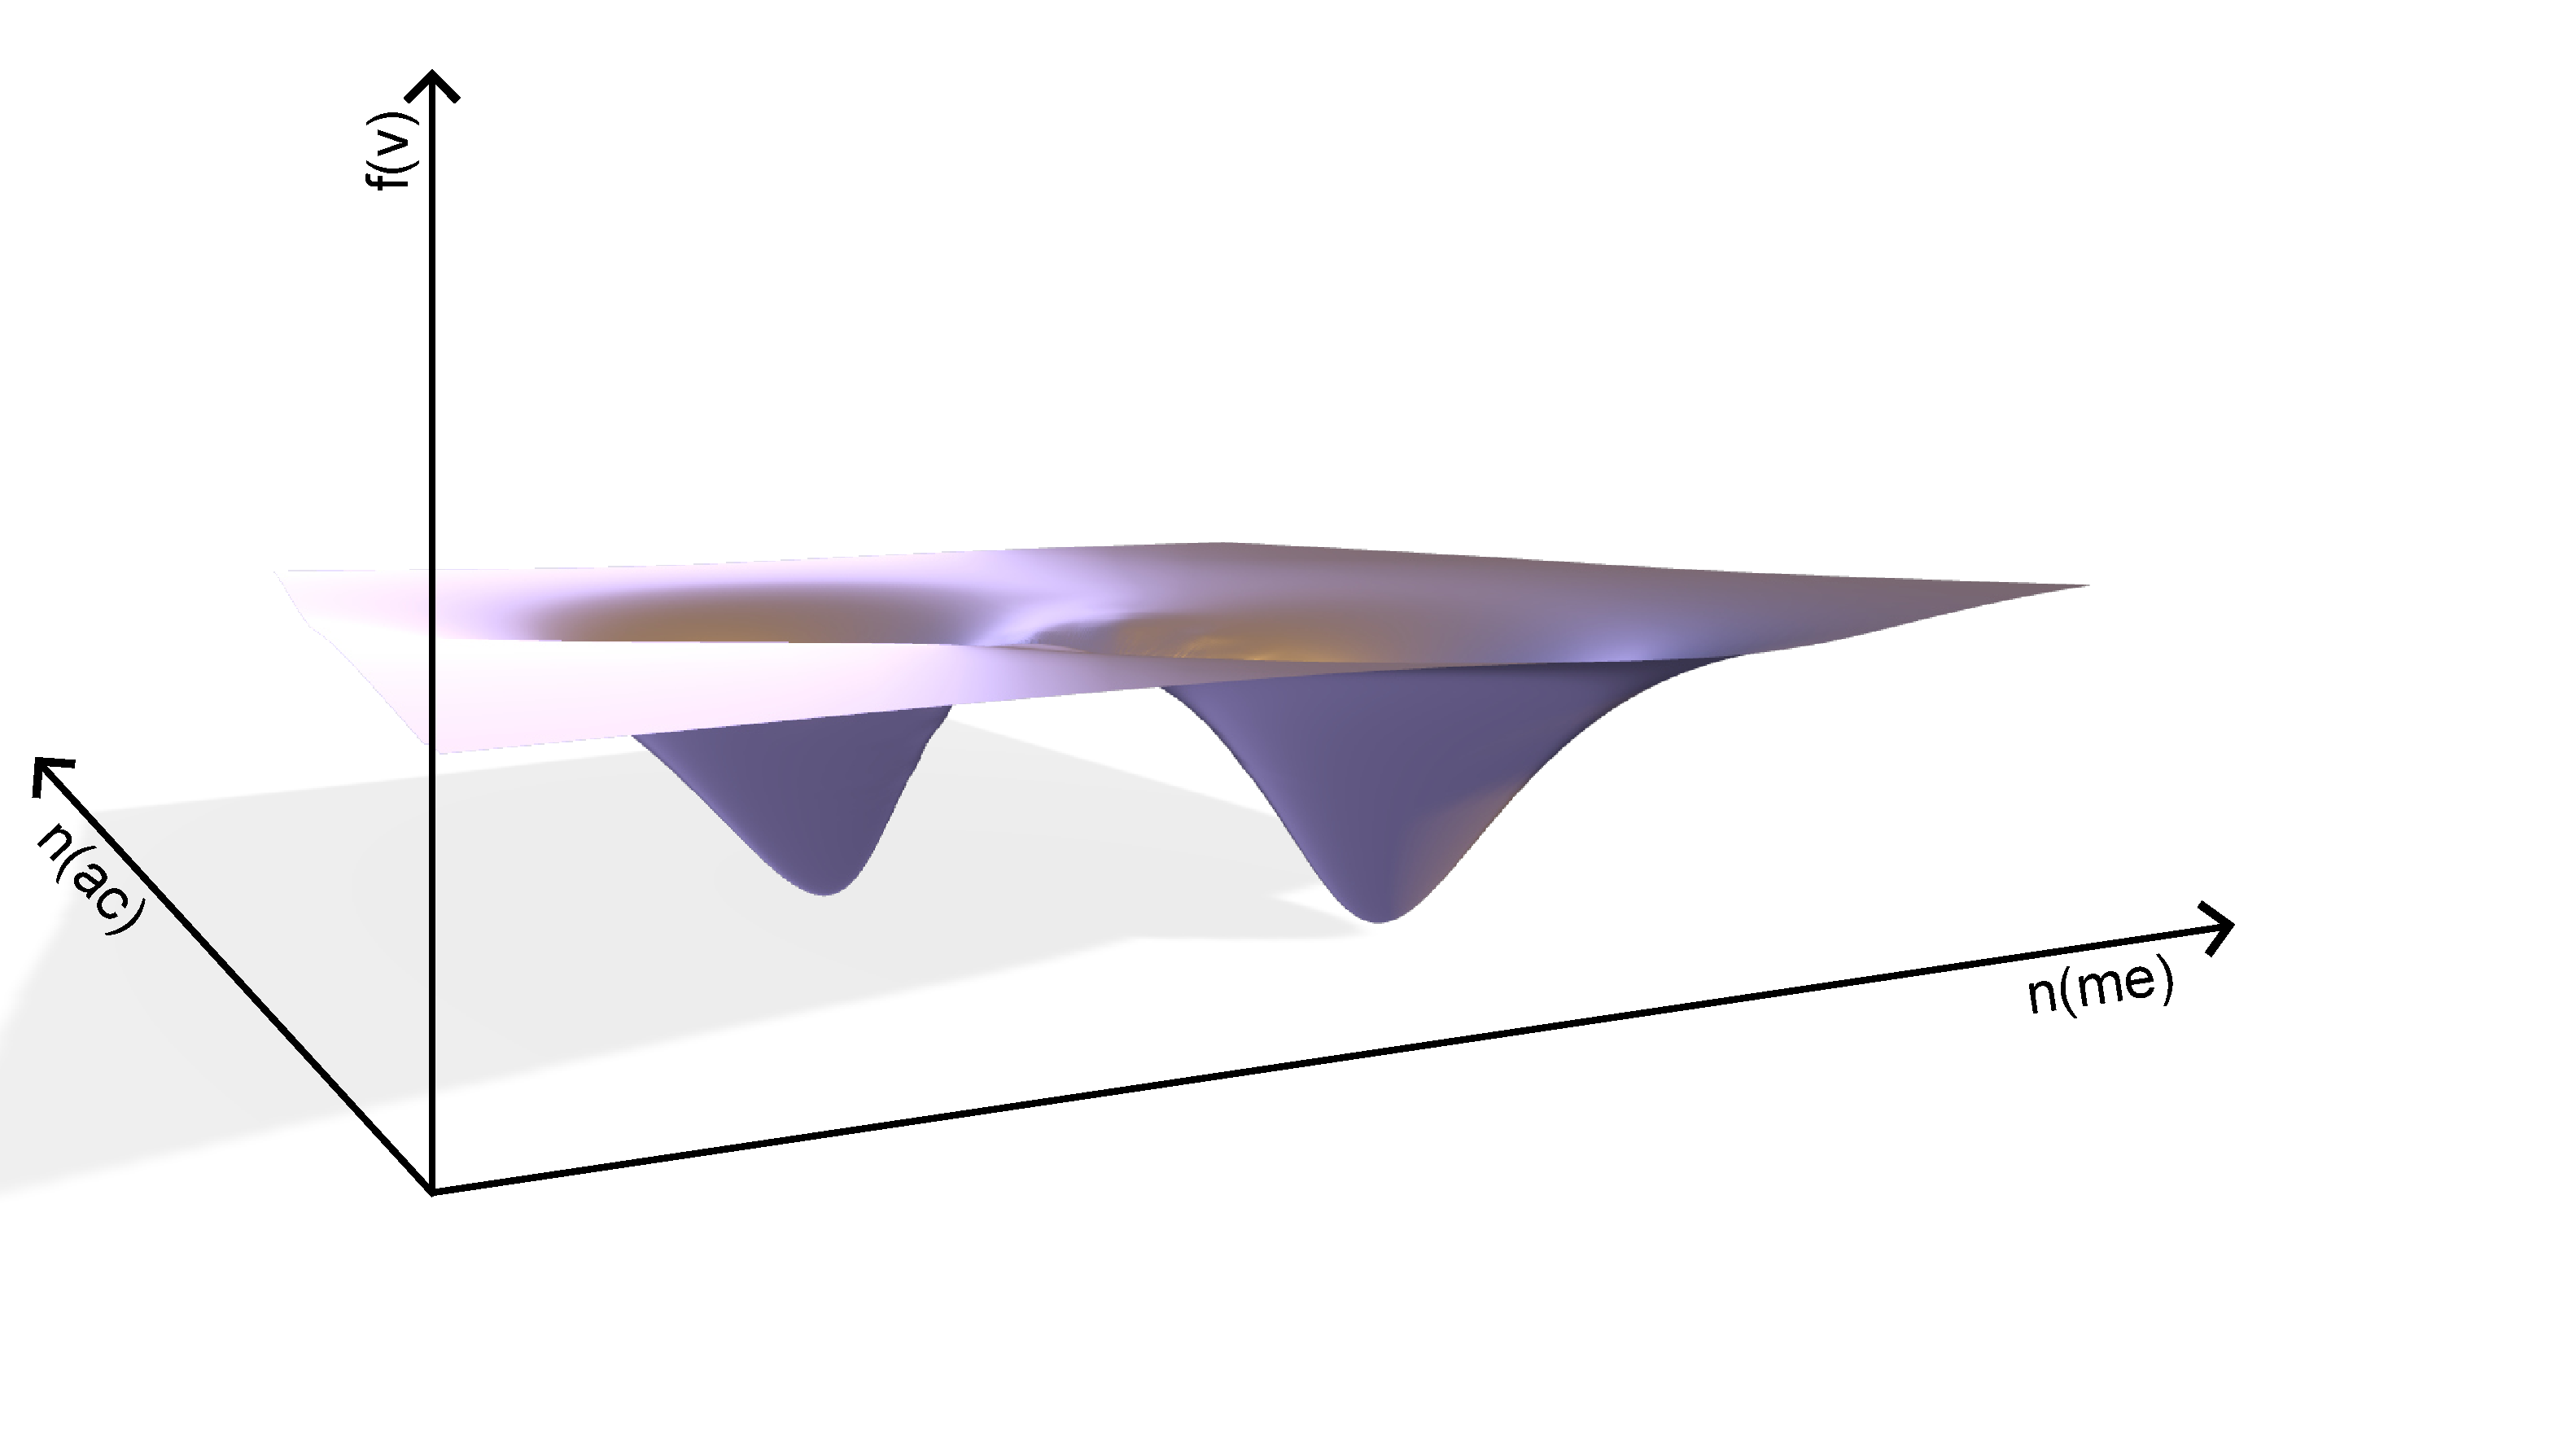
\includegraphics[width=\textwidth]{landscape_wAxes.pdf}
        %             \end{minipage}
        %             \begin{minipage}{0.19\textwidth}
        %                 \caption*{\small \textbf{(b)}}
        %             \end{minipage}
        %             \begin{minipage}{0.8\textwidth}
        %                 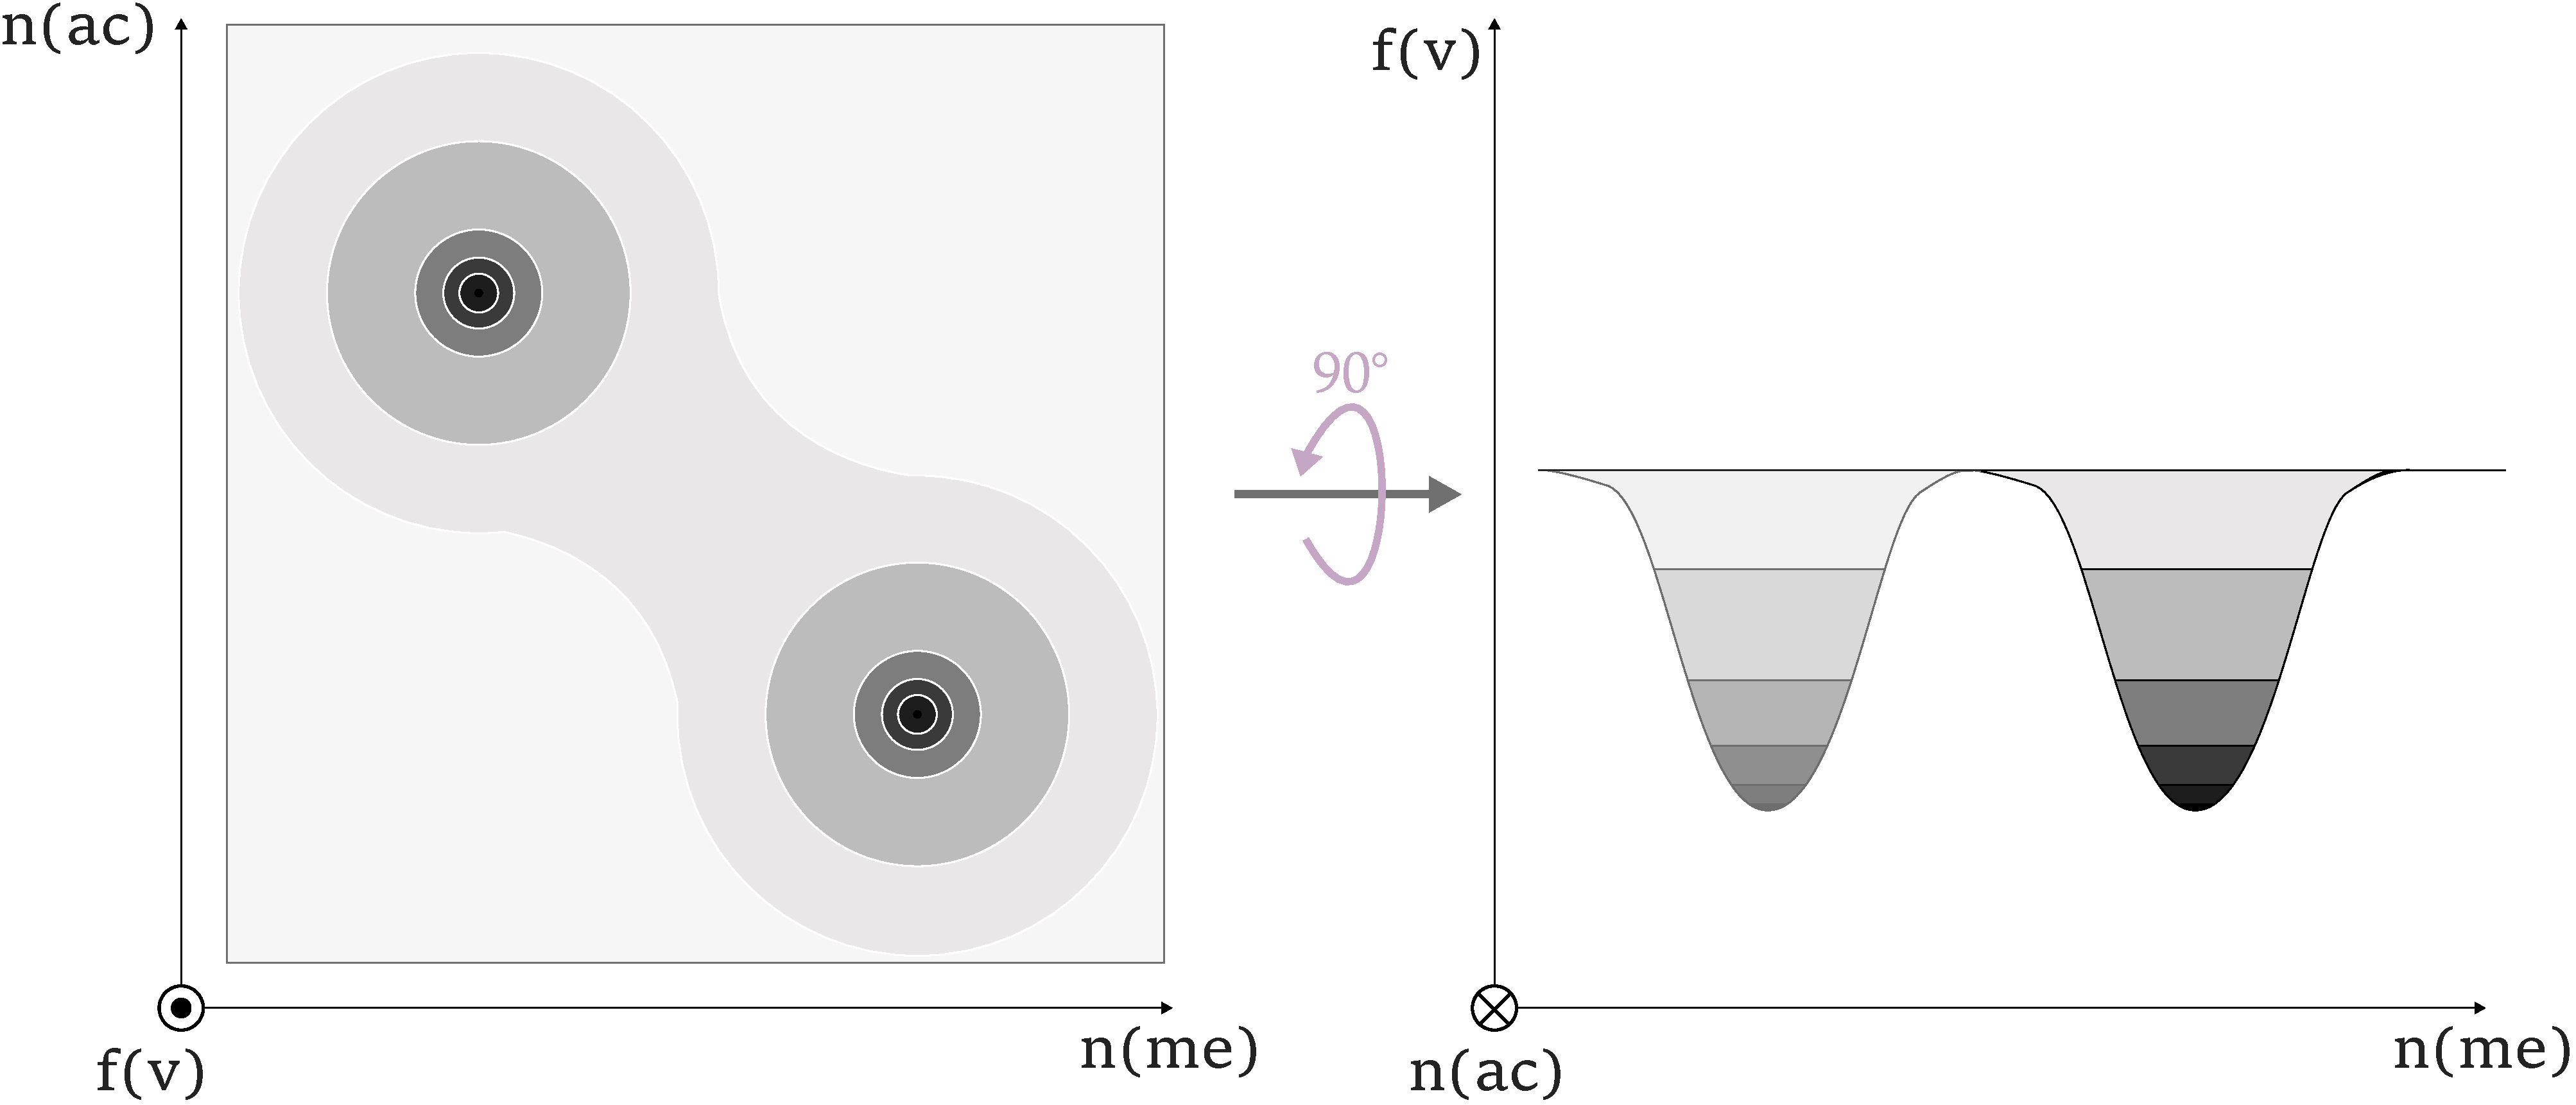
\includegraphics[width=\textwidth]{landscape_wAxes_2D.pdf}
        %             \end{minipage}
        %         \end{minipage}
        %         \caption{Simplified landscape example of a bistable system frozen in time. \textbf{(a)} 3D illustration modelled with Blender \cite{blender}. \textbf{(b)} 2D-projections along the indicated axes. The fix points in the basins are the most frequent configuration throughout a simulation. In most bistable systems, the basins are to be found close to the extrema of the $n(ac)$ and the $n(me)$ axes.}
        %         \label{img:fitnessLandscape}
        %     \end{figure}
        %     %

        %     %
        %     It is important to note that such a landscape is not constant in time. As the nucleosome string state changes, the effective activity of the enzymes changes, too. For instance, it is clear that a random \ac/ remover is more active the more \ac/ modifications are present on the string. This can even result in divergent effective enzyme sets throughout a simulation.
        %     %

        %     %
        %     \begin{itemize}
        %         {
        %             \color{red}
        %             \item ... explain the findings after counting the enzymatic activity in the cyclic case.
        %         }
        %     \end{itemize}
        %     %
        %
        % \subsection{Conditions for bistability}


        \subsection*{Enzyme set}
            %
            As was already found by Sneppen and Dodd, enzyme sets which exclusively contain enzymes with a maximum reach of 1 (next-neighbour) prevent robust bistability of the underlying dynamic histone PTM system.
            %

            %
            With cooperative enzymes present, bistability is quite often easily achieved. However, getting the system to perform bistable switching during a simulation can be quite challenging. With the cooperative remover enzymes being too effective in pertaining the complete macrostate, removing them from the enzyme set showed a massive increase in numbers of bistable switching events.
            %
        %
        %
        \subsection*{Association rate}
            %

            %
            The enzymes' association rate naturally is another factor which plays a role in bistability and bistable switching. The corresponding parameter that can be set in the enzyme rule set was not systematically analyzed. Nonetheless, the effective rate, meaning the actual binding event numbers, were recorded for the cyclic bistable case.
            %

            %
            A somewhat expected, yet very interesting, result was that the effective rates change during the simulation depending on the current macrostate.
            %

            %
            It remains unclear, in how far the aforementioned CME system is applicable to the case at hand given that the effective rates can hardly be predicted from the get-go.
            %

            %
        %
        %
        \subsection*{Dissociation rate}
            %

            %
            The dissociation rate was held unchanged for most of the simulations. Setting one and the same overly high dissociation rate that hardly competes with the enzymes' association rates reduces the overall noise in the system.
            %

            %
            Additionally, it was found in this work that a dissociation rate which is chosen too low can prevent bistability altogether.
            %

            %
            A variable dissociation rate would introduce high complexity into the system, as the number of relevant states would increase because the chromatin string would not only be sufficingly described by its modification pattern. Instead, the number and type of enzymes bound to the nucleosomes would also be an important factor.
            %

            %
            However, it could be biologically relevant to include low dissociation rates into the system, as for some histone PTM enzymes, the rate-limiting step turned out not to be the initial binding. For the human HAT enzyme, for instance, the rate-determining step is the transfer of the acetyl group onto K \cite{Tanner2000HATKinetics}.
            %
        %
        %
        \subsection*{Cooperative reach}
            %

            %
            In \ref{subsec:cooperativeEnzymeReach}, the impact of the cooperative enzymes' space value on bistability was analyzed. It turned out that for the present set of parameters, a space value of 4 to either side of the enzyme to be modified is enough in order to show bistability. Even though this value might only be valid for the exact parameters at hand, it is still an interesting finding that the enzymes' reach does not need to take the whole chromatin string into account in order to form a bistable system.
            %

            %
            Throughout this work, the cooperative enzymes' space was always kept equal to the left as to the right of the nucleosome to be modified. While this was a matter of convenience at first, it might also have some biological sense to it. As most enzymes are highly specific regarding the topological implications a substrate must present, it was shown in this work that some of this rigidity can be represented in the cooperative adders' structure without preventing bistability. It would be interesting to see, how far this rigidity could be increased before the system is not showing bistability any more.
            %

            %
        %
        %
        \subsection*{Chromatin cyclicity}
            %

            %
            As was extensively analyzed in this work, whether the chromatin string of a dynamic histone PTM system is cyclic or not has a huge impact on the presence or absence of bistable switching. As was discussed before, the system's bistability seems untouched from this property. However, bistable switching can be challenging to achieve consistently.
            %

            %
            Furthermore, bivalent switching could exclusively be consistently observed on non-cyclic strings. As soon as border effects are eliminated, the “STANDBY” state was hardly observed any more. As such, two major flaws are evident when assessing the biological significance of this form of bivalent switching:
            %

            %
            For one, as already mentioned before, the reversibility might be an undesired property in several contexts. It does not seem trivial to make bivalent switching, as found in this work, irreversible without adopting side effects.
            %

            %
            Secondly, the string borders are indispensable entities in order to achieve bivalent switching as found in this work. However, such borders which are “hard coded” into the system pose massive limitations to the applicability in real-life scenarios. At best, the issue of how gene transcription activity is regulated is shifted from histone modification dynamics to the question “How and where exactly are these barriers built around a gene?”. This results in little to no overall knowledge gain. It would be much more appropriate to find a way of inherently generating borders within a simulated chromatin string with the histone PTM machinery acting as a self-contained autoregulating system.\\
            %

            %
            As the aspect of cyclicity was analyzed in considerable depth, the findings about the bistable switching phenomenon in the two variants are summarized in the dedicated sections below.
            %
        %
        %
    %
    %
    \section{Mechanisms of bistable switching}
        %

        %
        \subsection{Non-cyclic case with cooperative removers}
            %

            %
            By means of the clues that were explained in \ref{sec:ResNonCyc} it seems appropriate to summarize the information in a general mechanism which shows how bistable switching can occur on a non-cyclic string by means of an enzyme rule set which contains cooperative enzymes. It is important to point out that this mechanism is not forcibly the only possibility of achieving bistable switching on a non-cyclic chromatin string. However, it was seen in numerous simulations and might help understand the crucial factors.
            %

            %
            \begin{figure}[htpb!]
                \centering
                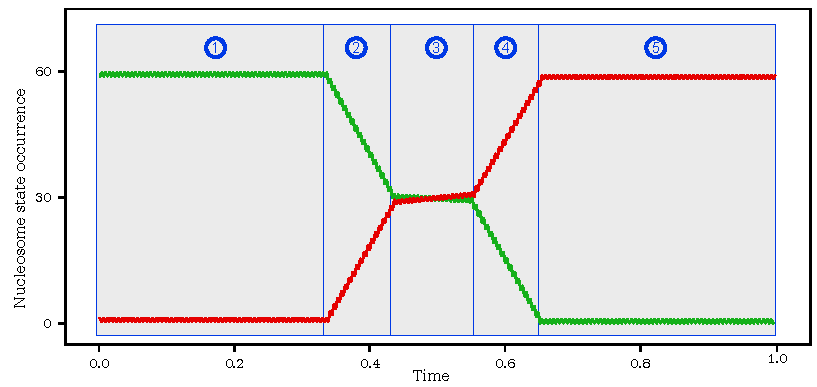
\includegraphics[width=\textwidth]{Discussion/nonCyclicMechanism_plot.pdf}
                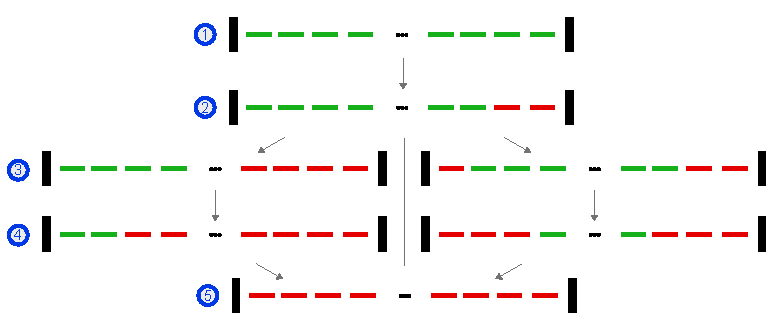
\includegraphics[width=\textwidth]{Discussion/nonCyclicMechanism_steps.pdf}
                \caption{Simplified de-noised graphical rundown of the macrostate switching process on a non-cyclic string with an enzyme set consisting of random adders, random removers, cooperative adders and cooperative removers. The upper figure is designed similarly to the plots showing the nucleosome state occurence throughout the simulation (see fig. \ref{img:nonCyclBistability_runPlot} for an example), starting with a fully acetylated chromatin string. The lower figure shows an exemplary nucleosome string containing the indicated nucleosome modification pattern based on the usual color code.}
                \label{img:DissNonCyclic}
            \end{figure}
            %

            %
            The general mechanism is schematized in fig. \ref{img:DissNonCyclic}. For reasons of simplicity, the starting string is a fully acetylated one. In this example, bistable switching is happening once, from \ac/ to \me/. Naturally, the same process could also happen in reversed order.
            %

            %
            During step \circled{1}, \ac/ stays the predominant modification. While some nucleosomes are demodified and might be methylated by a random adder, the cooperative removers keep the methylation modification from spreading considerably.
            %

            %
            At step \circled{2}, a small group of methylation marks was randomly added near a border of the string. Due to the rigidity of the cooperative removers, they can not read the outmost nucleosomes and, thus, cannot remove the \me/ modifications. Slowly and steadily, the \me/ modification can spread effectively inhibiting the cooperative \me/ remover because it must read one \ac/ mark on either side of the nucleosome to be removed.
            %

            %
            As the system is approaching step \circled{3}, what has previously been referred to as the saddle point, some simulations behave differently than others, depending on whether \me/ reached the string center from one or both borders of the string. If \me/ comes from one border and \ac/ dominates the other half of the string, the system can linger close to the saddle point for quite a while as the frontier between the \ac/ and \me/ areas are pushed back and forth. If \me/ is approaching from both string corners, generally, the \ac/ area is substituted by \me/ quite fast because the cooperative \ac/ removers become active as soon as their reach suffices in order to connect both \me/ areas.
            %

            %
            Step \circled{4} depicts the elimination of the \ac/ remainders. Depending on if \me/ has appeared on the other border or not up until now decides if the system might be able to revert soon.
            %

            %
            With step \circled{5} reached (which might not be always the case), \me/ is now the predominating modification.
            %
            %
        %
        %
        \subsection{Cyclic case without cooperative removers}
            %

            %
            For the cyclic case, unfortunately, no step-by-step mechanism can be proposed based on what was found in this work. However, the effective modification rates for an unmodified nucleosome in the three previously defined areas were calculated and are  shown in tab. \ref{tab:cyclBistabilities_modificationProb}. A comprehensive graphical representation of these data can be found in fig. \ref{img:DissCyclic}.
            %

            %
            \begin{figure}[htpb!]
                \centering
                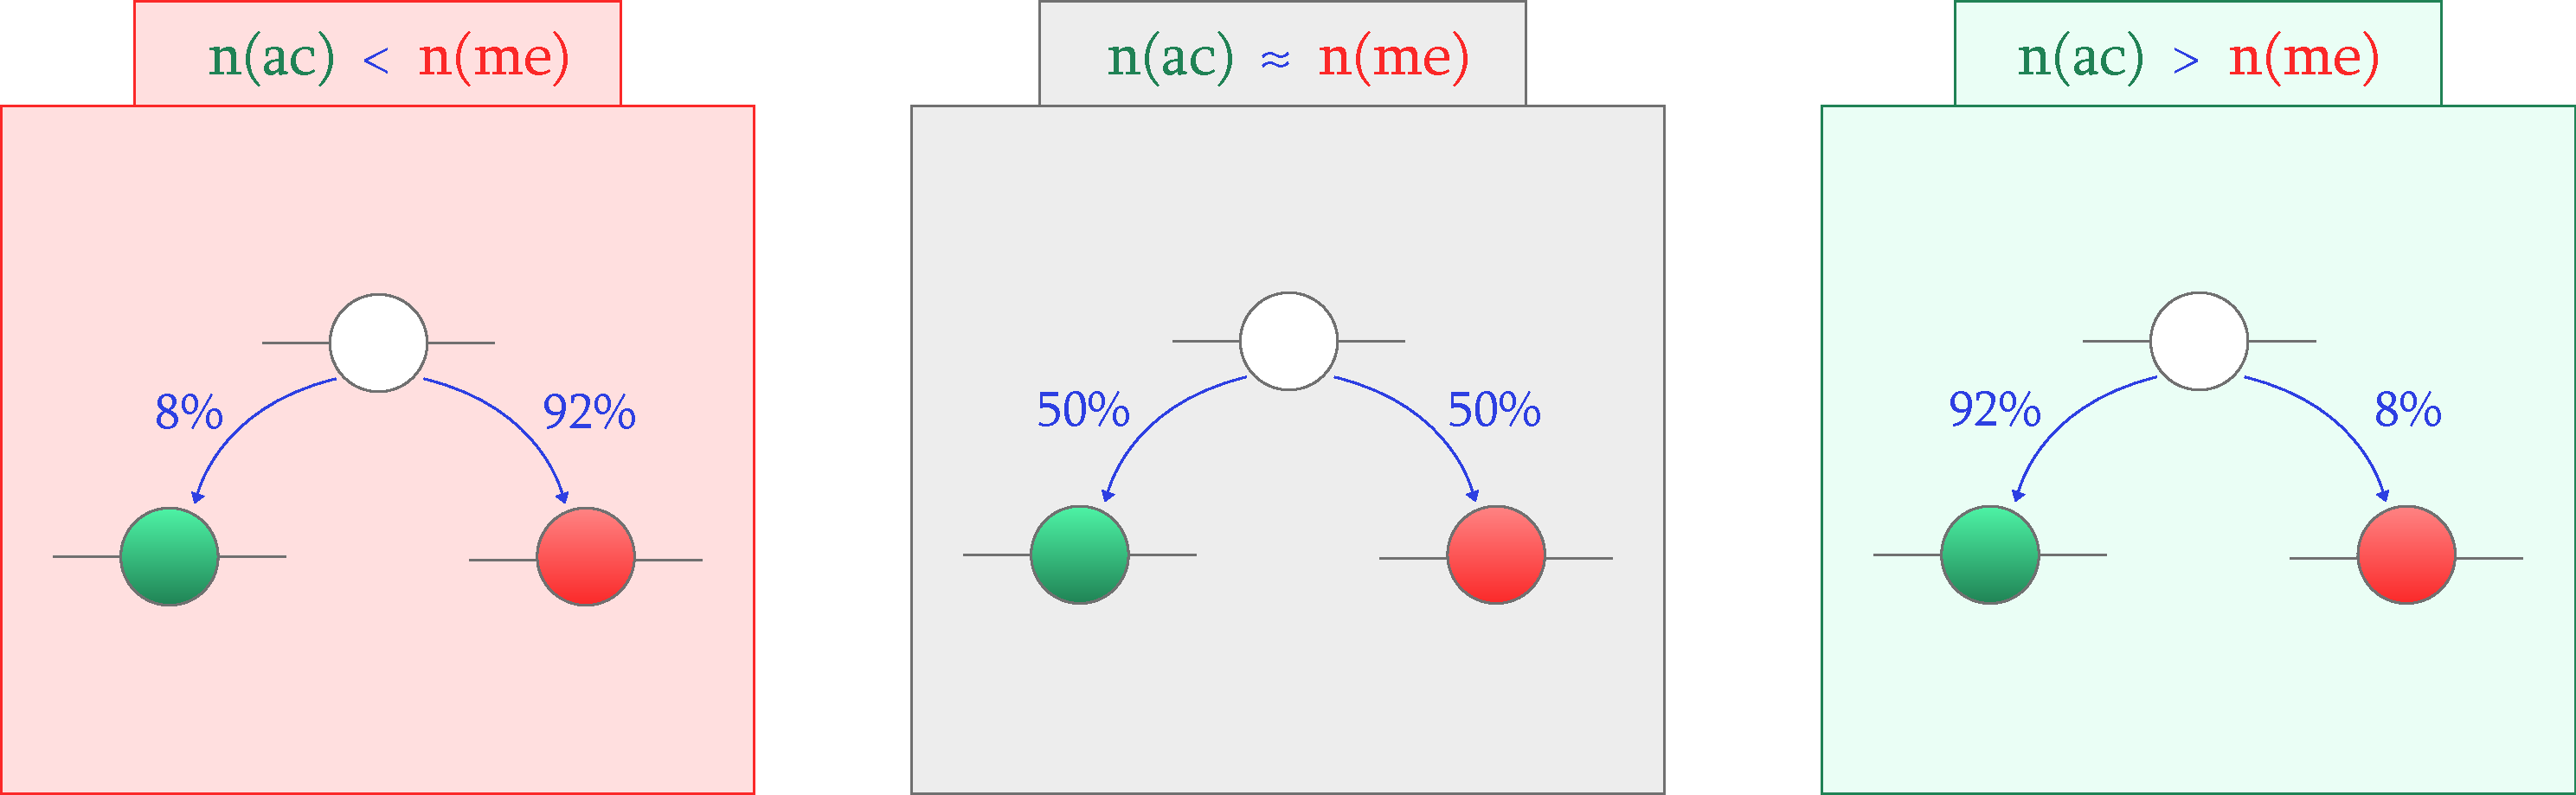
\includegraphics[width=\textwidth]{Discussion/cyclic_modRates_rounded.pdf} 
                \caption{Rounded modification probabilities of an unmodified nucleosome in the designated macrostate. The probabilities are based on calculations from 150 simulations with an average step number of about 600,000 each.}
                \label{img:DissCyclic}
            \end{figure}
            %

            %
            Based on these effective rates, it is quite clear that the system enters a random walk situation the closer it gets to the saddle point. With equal transition probabilities for an unmodified nucleosome to either \ac/ or \me/, the system can either be driven to a \me/ or an \ac/ macrostate. As the number of one specific modification increases, the respective cooperative adder enzymes gain a considerable amount of activity and drive the system further up to the respective complete (>90\%) macrostate.
            %

            %
            Unfortunately, with the incomplete analysis of the macrostate lengths at hand, no statement can be made about their systematics and the influence of other parameters on the length of a macrostate.
            %
        %
        %
    %
    %
%
%

\chapter{Outlook}
    \label{cha:outlook}
    %

    %
    As already stated in the discussion, this work partly serves as a preevaluation in order to provide some insight into the influential factors and their impact on bistability and macrostate switching. As such, it offers information that can be used for educated guesses in a next research step when it comes to systematically quantifying the effects of all the examined parameters and additional ones not analysed in this work.\\
    %

    %
    Other than that, during work on this thesis, some additional topics arose that could be worth addressment in the future.
    %

    %
    \begin{itemize}
        {
            \item \textbf{Macrostate length:} As discussed in \ref{subsec:macrostateLength}, it was not possible to gather sufficient data for reliable statistical analysis. With enough timely and spatial resources, however, this might be a topic worth exploring.
            \item \textbf{Variable dissociation rate:} Allowing considerably different dissociation rates per enzyme type could lead to results which are more suitable from a biological point of view \cite{Tanner2000HATKinetics}. Handling the complexity which arises with this undertaking will be a major challenge, but might be worth the effort.
            \item \textbf{Cooperative enzyme specificity:} As mentionned in the discussion, increasing the rigidity of cooperative enzymes might raise appeal on the biological side.
            \item \textbf{Implement 3D chromatin structure:} Schuettengruber et al. in \cite{schuettengruber2017genome} (p44f) explain that PREs (Polycomb response elements) are responsible for the chromatin forming loops (TADs = topologically associating domains) and are thus able to form large silenced areas of condensed chromatin. These 3D-formations are critical for HOX gene regulation. It is also known that many active gene promoters interact with their enhancers and other promoters in a 3D-fashion \cite{javierre2016lineage}. These findings suggest that it might be beneficial for \ed/ simulations to further explore possibilities to emulate fixed and dynamic 3D interactions within the nucleosome string.
        }
    \end{itemize}
    %
    %
%
%

%%%----------------------------------------------------------
\appendix                                         % appendix
%%%----------------------------------------------------------

\chapter{Specifications}
    \label{app:RunSpec}
    %

    %
    \section{Exemplary \ed/ run files}
        %
        \subsection{State file}
            \label{app:statefile}
            %
            \lstinputlisting[language=XMLnew]{xml/statefile.xml}
            %
        %
        %
        \subsection{Rule file}
            \label{app:rulefile}
            %
            \lstinputlisting[language=XMLnew]{xml/rulefile.xml}
            %
        %
        %
        \subsection{Param file}
            \label{app:paramfile}
            %
            \lstinputlisting[language=XMLnew]{xml/paramfile.xml}
            %
        %
        %
    %

    %
    \newpage
    \section{Summary of enzyme types}
        %

        %
        \begin{table}[htbp!]
            \caption{Summary of all the enzyme types that are referenced in this work. It is important to mention, that, for reasons of comprehensiveness, this table exemplarily only includes the rules which are in favour of acetylation (i.e. acetylation adders and methylation removers). However, every enzyme set used in this work is completely symmetrical. This means that if an enzyme set contains a linear acetylation adder it also contains a linear methylation adder at equal association and dissociation rates respectively and so forth.}
            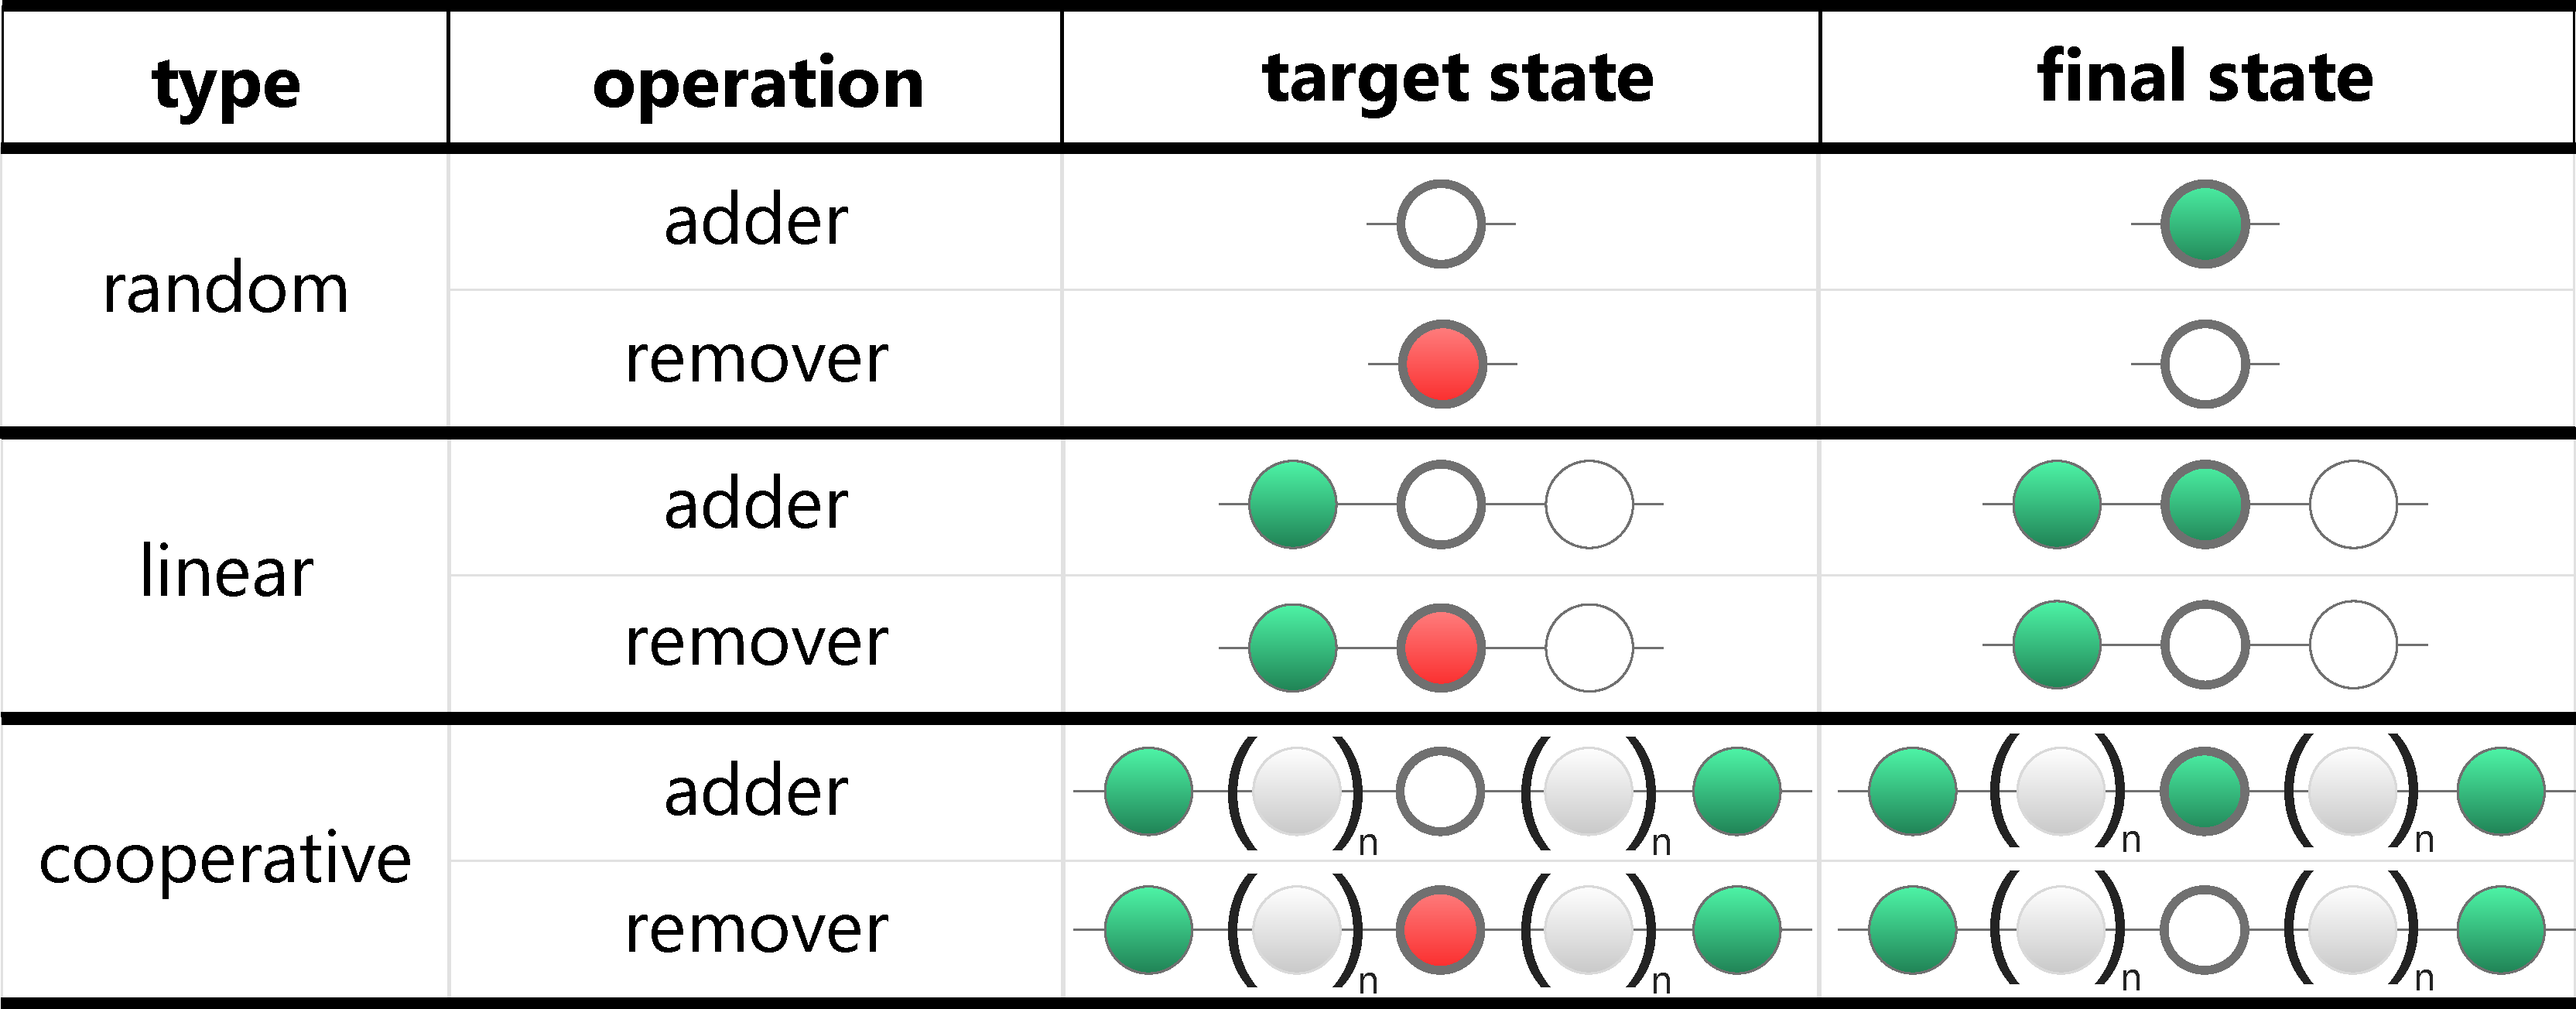
\includegraphics[width=\textwidth]{enzymes/table_newest.pdf}
            \label{img:enzymeTypeSummary}
        \end{table}
        %
        %
    %

    %
    % \section{Summary of simulation parameters}
    %     %

    %     %
    %     \begin{table}[htbp!]
    %         \caption{Summary of the simulation parameters explained in \ref{sec:simulationDetails} sorted by subsections in the 'Results' section.}
    %         \centering
    %         \begin{tabular}{lllllrr}
    %                                     &   &                               & coop?          & cyclic? & \multicolumn{1}{l}{diss?} & \multicolumn{1}{l}{simulation time}  \\
    %             \multicolumn{1}{r}{3.1} & ~ & long                          & no coop        & no      & 100000                    & 5                                    \\
    %             ~                       & ~ & short                         & no coop        & no      & 100000                    & 1                                    \\
    %             \multicolumn{1}{r}{3.2} & ~ & long                          & no coopRem     & no      & 100000                    & 5                                    \\
    %             ~                       & ~ & long                          & w coopRem      & no      & 100000                    & 5                                    \\
    %             ~                       & ~ & short                         & no coopRem     & no      & 100000                    & 1                                    \\
    %             ~                       & ~ & short                         & w coopRem      & no      & 100000                    & 1                                    \\
    %             \multicolumn{1}{r}{3.3} & ~ & long                          & no coopRem     & yes     & 100000                    & 20                                   \\
    %             ~                       & ~ & long                          & w coopRem      & yes     & 100000                    & 20                                   \\
    %             ~                       & ~ & short                         & no coopRem     & yes     & 100000                    & 8                                    \\
    %             ~                       & ~ & short                         & w coopRem      & yes     & 100000                    & 8                                    \\
    %             \multicolumn{1}{r}{3.4} & ~ & long                          & no coopRem     & yes     & 100000                    & 20                                   \\
    %             ~                       & ~ & long                          & no coopRem     & yes     & 100                       & 20                                   \\
    %             ~                       & ~ & short                         & no coopRem     & yes     & 100000                    & 6                                    \\
    %             ~                       & ~ & short                         & no coopRem     & yes     & 100                       & 6                                    \\
    %             \multicolumn{1}{r}{3.5} & ~ & maxReach0 (long)              & no coopRem     & yes     & 100000                    & 20                                   \\
    %             ~                       & ~ & maxReach1                     & no coopRem     & yes     & 100000                    & 20                                   \\
    %             ~                       & ~ & maxReach2                     & no coopRem     & yes     & 100000                    & 20                                   \\
    %             ~                       & ~ & maxReach3                     & no coopRem     & yes     & 100000                    & 20                                   \\
    %             ~                       & ~ & maxReach4                     & no coopRem     & yes     & 100000                    & 20                                   \\
    %             ~                       & ~ & maxReach5                     & no coopRem     & yes     & 100000                    & 20                                   \\
    %             ~                       & ~ & maxReach6                     & no coopRem     & yes     & 100000                    & 20                                   \\
    %             \multicolumn{1}{r}{3.6} & ~ & BivalentBistability
    %             (short) & no coopRem 2 K & yes     & 100000                    & 10                                   \\
    %             ~                       & ~ & FavBivalency (short)          & w coopRem      & yes     & 10000                     & 2                                    \\
    %             ~                       & ~ & FavTotal (short)              & w coopRem      & yes     & 10000                     & 2
    %         \end{tabular}
    %         \label{tab:simulationParametersSummary}
    %     \end{table}
    %     %
    %     %
    %
    %
%	% Run specifications
\chapter{Additional runs}
\label{app:additionalRuns}

\section{Additional runs from section \ref{sec:ResNon-cooperative}}
\label{app:additionalRuns1}

\begin{figure}[htbp!]
    \includeappendixrunplot{appendix_b/31_longRun_nonCyclic_highDiss_0_runHistoryPlot.pdf}
    \includeappendixrunplot{appendix_b/31_longRun_nonCyclic_highDiss_1_runHistoryPlot.pdf}
    \includeappendixrunplot{appendix_b/31_longRun_nonCyclic_highDiss_2_runHistoryPlot.pdf}
    \includeappendixrunplot{appendix_b/31_longRun_nonCyclic_highDiss_3_runHistoryPlot.pdf}
    % \includeappendixrunplot{appendix_b/31_longRun_nonCyclic_highDiss_4_runHistoryPlot.pdf}
    \caption{Runs from 3.1}
\end{figure}

\newpage
\section{Additional runs from section \ref{sec:ResNonCyc}}

\begin{figure}[htbp!]
    \includeappendixrunplot{appendix_b/32_longRun_nonCyclic_highDiss_wCoopRem_0_runHistoryPlot.pdf}
    \includeappendixrunplot{appendix_b/32_longRun_nonCyclic_highDiss_wCoopRem_1_runHistoryPlot.pdf}
    \includeappendixrunplot{appendix_b/32_longRun_nonCyclic_highDiss_wCoopRem_2_runHistoryPlot.pdf}
    \includeappendixrunplot{appendix_b/32_longRun_nonCyclic_highDiss_wCoopRem_3_runHistoryPlot.pdf}
    % \includeappendixrunplot{appendix_b/32_longRun_nonCyclic_highDiss_wCoopRem_4_runHistoryPlot.pdf}
    \caption{Runs from 3.2}
\end{figure}	% Additional runs
\chapter{Source Code}
    \label{app:SourceCode}
    %

    %
    \section{Used software}
        %
        The source code for the used simulation software, \ed/, can be found at \cite{Herbig2021EpiDynaST}.
        %
    %
    %
    \section{Data and scripts}
        %
        The data generated for this thesis as well as the evaluation scripts can be found at \cite{Krecké2021}.
        %
    %
    %
    \section{Thesis \LaTeX{} code}
        %
        The \LaTeX{} source code for this very thesis can be found at \cite{Krecké2021Thesis}.
        %
    %
    %
%
%




	% Source Code
% \chapter{\latex Source Code}
\label{app:SourceCode}

	% source text of this document

%%%----------------------------------------------------------
\MakeBibliography                        				% references
%%%----------------------------------------------------------

%%% special page for checking print size --------------------
% \chapter*{Check Final Print Size}

\begin{center}
{\Large --- Check final print size! ---}

\bigskip

\calibrationbox{100}{50} % width/height of box in mm

\bigskip

{\Large --- Remove this page after printing! ---}

\end{center}



%%%----------------------------------------------------------
\end{document}
%%%----------------------------------------------------------